\documentclass[twoside]{book}

% Packages required by doxygen
\usepackage{fixltx2e}
\usepackage{calc}
\usepackage{doxygen}
\usepackage[export]{adjustbox} % also loads graphicx
\usepackage{graphicx}
\usepackage[utf8]{inputenc}
\usepackage{makeidx}
\usepackage{multicol}
\usepackage{multirow}
\PassOptionsToPackage{warn}{textcomp}
\usepackage{textcomp}
\usepackage[nointegrals]{wasysym}
\usepackage[table]{xcolor}

% Font selection
\usepackage[T1]{fontenc}
\usepackage[scaled=.90]{helvet}
\usepackage{courier}
\usepackage{amssymb}
\usepackage{sectsty}
\renewcommand{\familydefault}{\sfdefault}
\allsectionsfont{%
  \fontseries{bc}\selectfont%
  \color{darkgray}%
}
\renewcommand{\DoxyLabelFont}{%
  \fontseries{bc}\selectfont%
  \color{darkgray}%
}
\newcommand{\+}{\discretionary{\mbox{\scriptsize$\hookleftarrow$}}{}{}}

% Page & text layout
\usepackage{geometry}
\geometry{%
  a4paper,%
  top=2.5cm,%
  bottom=2.5cm,%
  left=2.5cm,%
  right=2.5cm%
}
\tolerance=750
\hfuzz=15pt
\hbadness=750
\setlength{\emergencystretch}{15pt}
\setlength{\parindent}{0cm}
\setlength{\parskip}{3ex plus 2ex minus 2ex}
\makeatletter
\renewcommand{\paragraph}{%
  \@startsection{paragraph}{4}{0ex}{-1.0ex}{1.0ex}{%
    \normalfont\normalsize\bfseries\SS@parafont%
  }%
}
\renewcommand{\subparagraph}{%
  \@startsection{subparagraph}{5}{0ex}{-1.0ex}{1.0ex}{%
    \normalfont\normalsize\bfseries\SS@subparafont%
  }%
}
\makeatother

% Headers & footers
\usepackage{fancyhdr}
\pagestyle{fancyplain}
\fancyhead[LE]{\fancyplain{}{\bfseries\thepage}}
\fancyhead[CE]{\fancyplain{}{}}
\fancyhead[RE]{\fancyplain{}{\bfseries\leftmark}}
\fancyhead[LO]{\fancyplain{}{\bfseries\rightmark}}
\fancyhead[CO]{\fancyplain{}{}}
\fancyhead[RO]{\fancyplain{}{\bfseries\thepage}}
\fancyfoot[LE]{\fancyplain{}{}}
\fancyfoot[CE]{\fancyplain{}{}}
\fancyfoot[RE]{\fancyplain{}{\bfseries\scriptsize Generated by Doxygen }}
\fancyfoot[LO]{\fancyplain{}{\bfseries\scriptsize Generated by Doxygen }}
\fancyfoot[CO]{\fancyplain{}{}}
\fancyfoot[RO]{\fancyplain{}{}}
\renewcommand{\footrulewidth}{0.4pt}
\renewcommand{\chaptermark}[1]{%
  \markboth{#1}{}%
}
\renewcommand{\sectionmark}[1]{%
  \markright{\thesection\ #1}%
}

% Indices & bibliography
\usepackage{natbib}
\usepackage[titles]{tocloft}
\setcounter{tocdepth}{3}
\setcounter{secnumdepth}{5}
\makeindex

% Hyperlinks (required, but should be loaded last)
\usepackage{ifpdf}
\ifpdf
  \usepackage[pdftex,pagebackref=true]{hyperref}
\else
  \usepackage[ps2pdf,pagebackref=true]{hyperref}
\fi
\hypersetup{%
  colorlinks=true,%
  linkcolor=blue,%
  citecolor=blue,%
  unicode%
}

% Custom commands
\newcommand{\clearemptydoublepage}{%
  \newpage{\pagestyle{empty}\cleardoublepage}%
}

\usepackage{caption}
\captionsetup{labelsep=space,justification=centering,font={bf},singlelinecheck=off,skip=4pt,position=top}

%===== C O N T E N T S =====

\begin{document}

% Titlepage & ToC
\hypersetup{pageanchor=false,
             bookmarksnumbered=true,
             pdfencoding=unicode
            }
\pagenumbering{roman}
\begin{titlepage}
\vspace*{7cm}
\begin{center}%
{\Large goldboard4 }\\
\vspace*{1cm}
{\large Generated by Doxygen 1.8.11}\\
\end{center}
\end{titlepage}
\clearemptydoublepage
\tableofcontents
\clearemptydoublepage
\pagenumbering{arabic}
\hypersetup{pageanchor=true}

%--- Begin generated contents ---
\chapter{Module Index}
\section{Modules}
Here is a list of all modules\+:\begin{DoxyCompactList}
\item \contentsline{section}{U\+A\+RT Library}{\pageref{group__pfleury__uart}}{}
\end{DoxyCompactList}

\chapter{Hierarchical Index}
\section{Class Hierarchy}
This inheritance list is sorted roughly, but not completely, alphabetically\+:\begin{DoxyCompactList}
\item \contentsline{section}{Block}{\pageref{struct_block}}{}
\item \contentsline{section}{B\+N\+O055}{\pageref{class_b_n_o055}}{}
\item \contentsline{section}{C\+M\+P\+S03}{\pageref{class_c_m_p_s03}}{}
\item \contentsline{section}{Goldboard4}{\pageref{class_goldboard4}}{}
\item \contentsline{section}{H\+C05}{\pageref{class_h_c05}}{}
\item \contentsline{section}{Link\+I2C}{\pageref{class_link_i2_c}}{}
\item \contentsline{section}{Link\+U\+A\+RT}{\pageref{class_link_u_a_r_t}}{}
\item \contentsline{section}{Motor}{\pageref{class_motor}}{}
\item \contentsline{section}{Stream\+:\+:Multi\+Target}{\pageref{struct_stream_1_1_multi_target}}{}
\item \contentsline{section}{P\+C\+F8574A}{\pageref{class_p_c_f8574_a}}{}
\item \contentsline{section}{Print}{\pageref{class_print}}{}
\begin{DoxyCompactList}
\item \contentsline{section}{Software\+Serial}{\pageref{class_software_serial}}{}
\item \contentsline{section}{Stream}{\pageref{class_stream}}{}
\begin{DoxyCompactList}
\item \contentsline{section}{Two\+Wire}{\pageref{class_two_wire}}{}
\end{DoxyCompactList}
\end{DoxyCompactList}
\item \contentsline{section}{Printable}{\pageref{class_printable}}{}
\item \contentsline{section}{S\+R\+F08}{\pageref{class_s_r_f08}}{}
\item \contentsline{section}{T\+Pixy$<$ Link\+Type $>$}{\pageref{class_t_pixy}}{}
\item \contentsline{section}{T\+Pixy$<$ Link\+I2C $>$}{\pageref{class_t_pixy}}{}
\item \contentsline{section}{usring}{\pageref{classusring}}{}
\item \contentsline{section}{V\+L53\+L0X}{\pageref{class_v_l53_l0_x}}{}
\end{DoxyCompactList}

\chapter{Class Index}
\section{Class List}
Here are the classes, structs, unions and interfaces with brief descriptions\+:\begin{DoxyCompactList}
\item\contentsline{section}{\hyperlink{struct_block}{Block} }{\pageref{struct_block}}{}
\item\contentsline{section}{\hyperlink{class_b_n_o055}{B\+N\+O055} }{\pageref{class_b_n_o055}}{}
\item\contentsline{section}{\hyperlink{class_c_m_p_s03}{C\+M\+P\+S03} }{\pageref{class_c_m_p_s03}}{}
\item\contentsline{section}{\hyperlink{class_goldboard4}{Goldboard4} }{\pageref{class_goldboard4}}{}
\item\contentsline{section}{\hyperlink{class_h_c05}{H\+C05} }{\pageref{class_h_c05}}{}
\item\contentsline{section}{\hyperlink{class_link_i2_c}{Link\+I2C} }{\pageref{class_link_i2_c}}{}
\item\contentsline{section}{\hyperlink{class_link_u_a_r_t}{Link\+U\+A\+RT} }{\pageref{class_link_u_a_r_t}}{}
\item\contentsline{section}{\hyperlink{class_motor}{Motor} }{\pageref{class_motor}}{}
\item\contentsline{section}{\hyperlink{struct_stream_1_1_multi_target}{Stream\+::\+Multi\+Target} }{\pageref{struct_stream_1_1_multi_target}}{}
\item\contentsline{section}{\hyperlink{class_p_c_f8574_a}{P\+C\+F8574A} }{\pageref{class_p_c_f8574_a}}{}
\item\contentsline{section}{\hyperlink{class_print}{Print} }{\pageref{class_print}}{}
\item\contentsline{section}{\hyperlink{class_printable}{Printable} }{\pageref{class_printable}}{}
\item\contentsline{section}{\hyperlink{class_software_serial}{Software\+Serial} }{\pageref{class_software_serial}}{}
\item\contentsline{section}{\hyperlink{class_s_r_f08}{S\+R\+F08} }{\pageref{class_s_r_f08}}{}
\item\contentsline{section}{\hyperlink{class_stream}{Stream} }{\pageref{class_stream}}{}
\item\contentsline{section}{\hyperlink{class_t_pixy}{T\+Pixy$<$ Link\+Type $>$} }{\pageref{class_t_pixy}}{}
\item\contentsline{section}{\hyperlink{class_two_wire}{Two\+Wire} }{\pageref{class_two_wire}}{}
\item\contentsline{section}{\hyperlink{classusring}{usring} }{\pageref{classusring}}{}
\item\contentsline{section}{\hyperlink{class_v_l53_l0_x}{V\+L53\+L0X} }{\pageref{class_v_l53_l0_x}}{}
\end{DoxyCompactList}

\chapter{File Index}
\section{File List}
Here is a list of all documented files with brief descriptions\+:\begin{DoxyCompactList}
\item\contentsline{section}{/home/alex/workspace/goldboard4/libs/goldboard4/{\bfseries C\+M\+P\+S03.\+h} }{\pageref{_c_m_p_s03_8h}}{}
\item\contentsline{section}{/home/alex/workspace/goldboard4/libs/goldboard4/{\bfseries config.\+h} }{\pageref{config_8h}}{}
\item\contentsline{section}{/home/alex/workspace/goldboard4/libs/goldboard4/{\bfseries global.\+h} }{\pageref{global_8h}}{}
\item\contentsline{section}{/home/alex/workspace/goldboard4/libs/goldboard4/{\bfseries Goldboard4.\+h} }{\pageref{_goldboard4_8h}}{}
\item\contentsline{section}{/home/alex/workspace/goldboard4/libs/goldboard4/\hyperlink{i2c_8h}{i2c.\+h} \\*I2\+C-\/\+Treiber, derzeit nur Master, interruptbasiert }{\pageref{i2c_8h}}{}
\item\contentsline{section}{/home/alex/workspace/goldboard4/libs/goldboard4/{\bfseries Motor.\+h} }{\pageref{_motor_8h}}{}
\item\contentsline{section}{/home/alex/workspace/goldboard4/libs/goldboard4/{\bfseries new.\+h} }{\pageref{new_8h}}{}
\item\contentsline{section}{/home/alex/workspace/goldboard4/libs/goldboard4/{\bfseries P\+C\+F8574\+A.\+h} }{\pageref{_p_c_f8574_a_8h}}{}
\item\contentsline{section}{/home/alex/workspace/goldboard4/libs/goldboard4/{\bfseries pin\+\_\+configuration.\+h} }{\pageref{pin__configuration_8h}}{}
\item\contentsline{section}{/home/alex/workspace/goldboard4/libs/goldboard4/{\bfseries Pixy\+I2\+C.\+h} }{\pageref{_pixy_i2_c_8h}}{}
\item\contentsline{section}{/home/alex/workspace/goldboard4/libs/goldboard4/{\bfseries Pixy\+U\+A\+R\+T.\+h} }{\pageref{_pixy_u_a_r_t_8h}}{}
\item\contentsline{section}{/home/alex/workspace/goldboard4/libs/goldboard4/{\bfseries Print.\+h} }{\pageref{_print_8h}}{}
\item\contentsline{section}{/home/alex/workspace/goldboard4/libs/goldboard4/{\bfseries Printable.\+h} }{\pageref{_printable_8h}}{}
\item\contentsline{section}{/home/alex/workspace/goldboard4/libs/goldboard4/{\bfseries Serial.\+h} }{\pageref{_serial_8h}}{}
\item\contentsline{section}{/home/alex/workspace/goldboard4/libs/goldboard4/{\bfseries Soft\+I2\+C\+Master.\+h} }{\pageref{_soft_i2_c_master_8h}}{}
\item\contentsline{section}{/home/alex/workspace/goldboard4/libs/goldboard4/{\bfseries S\+R\+F08.\+h} }{\pageref{_s_r_f08_8h}}{}
\item\contentsline{section}{/home/alex/workspace/goldboard4/libs/goldboard4/{\bfseries Stream.\+h} }{\pageref{_stream_8h}}{}
\item\contentsline{section}{/home/alex/workspace/goldboard4/libs/goldboard4/{\bfseries T\+Pixy.\+h} }{\pageref{_t_pixy_8h}}{}
\item\contentsline{section}{/home/alex/workspace/goldboard4/libs/goldboard4/{\bfseries twi.\+h} }{\pageref{twi_8h}}{}
\item\contentsline{section}{/home/alex/workspace/goldboard4/libs/goldboard4/{\bfseries uart.\+h} }{\pageref{uart_8h}}{}
\item\contentsline{section}{/home/alex/workspace/goldboard4/libs/goldboard4/{\bfseries usring.\+h} }{\pageref{usring_8h}}{}
\item\contentsline{section}{/home/alex/workspace/goldboard4/libs/goldboard4/{\bfseries V\+L53\+L0\+X.\+h} }{\pageref{_v_l53_l0_x_8h}}{}
\item\contentsline{section}{/home/alex/workspace/goldboard4/libs/goldboard4/{\bfseries W\+Character.\+h} }{\pageref{_w_character_8h}}{}
\item\contentsline{section}{/home/alex/workspace/goldboard4/libs/goldboard4/{\bfseries Wire.\+h} }{\pageref{_wire_8h}}{}
\item\contentsline{section}{/home/alex/workspace/goldboard4/libs/goldboard4/{\bfseries wiring\+\_\+private.\+h} }{\pageref{wiring__private_8h}}{}
\item\contentsline{section}{/home/alex/workspace/goldboard4/libs/goldboard4/{\bfseries W\+String.\+h} }{\pageref{_w_string_8h}}{}
\end{DoxyCompactList}

\chapter{Module Documentation}
\hypertarget{group__pfleury__uart}{}\section{U\+A\+RT Library}
\label{group__pfleury__uart}\index{U\+A\+R\+T Library@{U\+A\+R\+T Library}}


Interrupt U\+A\+RT library using the built-\/in U\+A\+RT with transmit and receive circular buffers.  


\subsection*{Macros}
\begin{DoxyCompactItemize}
\item 
\#define \hyperlink{group__pfleury__uart_ga367ff7b5de225ed936a63239ad4adb0b}{U\+A\+R\+T\+\_\+\+B\+A\+U\+D\+\_\+\+S\+E\+L\+E\+CT}(baud\+Rate,  xtal\+Cpu)~(((xtal\+Cpu) + 8\+U\+L $\ast$ (baud\+Rate)) / (16\+U\+L $\ast$ (baud\+Rate)) -\/1\+U\+L)
\begin{DoxyCompactList}\small\item\em U\+A\+RT Baudrate Expression. \end{DoxyCompactList}\item 
\#define \hyperlink{group__pfleury__uart_ga1a02d45130520cb651ab313e69039382}{U\+A\+R\+T\+\_\+\+B\+A\+U\+D\+\_\+\+S\+E\+L\+E\+C\+T\+\_\+\+D\+O\+U\+B\+L\+E\+\_\+\+S\+P\+E\+ED}(baud\+Rate,  xtal\+Cpu)~( ((((xtal\+Cpu) + 4\+U\+L $\ast$ (baud\+Rate)) / (8\+U\+L $\ast$ (baud\+Rate)) -\/1\+U\+L)) $\vert$ 0x8000)
\begin{DoxyCompactList}\small\item\em U\+A\+RT Baudrate Expression for A\+Tmega double speed mode. \end{DoxyCompactList}\item 
\#define \hyperlink{group__pfleury__uart_ga5bdd6772c246436bb14377095de79b31}{U\+A\+R\+T\+\_\+\+R\+X\+\_\+\+B\+U\+F\+F\+E\+R\+\_\+\+S\+I\+ZE}~32
\item 
\#define \hyperlink{group__pfleury__uart_ga05f5d709605c6317c97e4974bec3402a}{U\+A\+R\+T\+\_\+\+T\+X\+\_\+\+B\+U\+F\+F\+E\+R\+\_\+\+S\+I\+ZE}~32
\item 
\#define {\bfseries U\+A\+R\+T\+\_\+\+F\+R\+A\+M\+E\+\_\+\+E\+R\+R\+OR}~0x1000              /$\ast$ Framing Error by U\+A\+R\+T       $\ast$/\hypertarget{group__pfleury__uart_gabcdb1041d763560cd8f8e722370dfd37}{}\label{group__pfleury__uart_gabcdb1041d763560cd8f8e722370dfd37}

\item 
\#define {\bfseries U\+A\+R\+T\+\_\+\+O\+V\+E\+R\+R\+U\+N\+\_\+\+E\+R\+R\+OR}~0x0800              /$\ast$ Overrun condition by U\+A\+R\+T   $\ast$/\hypertarget{group__pfleury__uart_ga3183177e3613d8785d8cc8516931beb6}{}\label{group__pfleury__uart_ga3183177e3613d8785d8cc8516931beb6}

\item 
\#define {\bfseries U\+A\+R\+T\+\_\+\+P\+A\+R\+I\+T\+Y\+\_\+\+E\+R\+R\+OR}~0x0400              /$\ast$ Parity Error by U\+A\+R\+T        $\ast$/\hypertarget{group__pfleury__uart_ga946e3d317937e003d2057bf19e96dd1d}{}\label{group__pfleury__uart_ga946e3d317937e003d2057bf19e96dd1d}

\item 
\#define {\bfseries U\+A\+R\+T\+\_\+\+B\+U\+F\+F\+E\+R\+\_\+\+O\+V\+E\+R\+F\+L\+OW}~0x0200              /$\ast$ receive ringbuffer overflow $\ast$/\hypertarget{group__pfleury__uart_ga94758f3dad6864703b7417d3e40f11df}{}\label{group__pfleury__uart_ga94758f3dad6864703b7417d3e40f11df}

\item 
\#define {\bfseries U\+A\+R\+T\+\_\+\+N\+O\+\_\+\+D\+A\+TA}~0x0100              /$\ast$ no receive data available   $\ast$/\hypertarget{group__pfleury__uart_ga77ba544d423ff42d400220a05303f268}{}\label{group__pfleury__uart_ga77ba544d423ff42d400220a05303f268}

\item 
\#define \hyperlink{group__pfleury__uart_gae9e143569df2285379bc55f9f5595bf9}{uart\+\_\+puts\+\_\+P}(\+\_\+\+\_\+s)~\hyperlink{group__pfleury__uart_ga6d78b6744db6232f52b4616402036c2f}{uart\+\_\+puts\+\_\+p}(P\+S\+TR(\+\_\+\+\_\+s))\hypertarget{group__pfleury__uart_gae9e143569df2285379bc55f9f5595bf9}{}\label{group__pfleury__uart_gae9e143569df2285379bc55f9f5595bf9}

\begin{DoxyCompactList}\small\item\em Macro to automatically put a string constant into program memory. \end{DoxyCompactList}\item 
\#define \hyperlink{group__pfleury__uart_gaabd7a5b0c15611ee9ecb2873cc9ee87a}{uart1\+\_\+puts\+\_\+P}(\+\_\+\+\_\+s)~\hyperlink{group__pfleury__uart_ga1e8074d0a2d5922601c5db2f9777ba79}{uart1\+\_\+puts\+\_\+p}(P\+S\+TR(\+\_\+\+\_\+s))\hypertarget{group__pfleury__uart_gaabd7a5b0c15611ee9ecb2873cc9ee87a}{}\label{group__pfleury__uart_gaabd7a5b0c15611ee9ecb2873cc9ee87a}

\begin{DoxyCompactList}\small\item\em Macro to automatically put a string constant into program memory. \end{DoxyCompactList}\end{DoxyCompactItemize}
\subsection*{Functions}
\begin{DoxyCompactItemize}
\item 
void \hyperlink{group__pfleury__uart_gac19a76bb7d446125734a67f9f4b68991}{uart\+\_\+init} (unsigned int baudrate)
\begin{DoxyCompactList}\small\item\em Initialize U\+A\+RT and set baudrate. \end{DoxyCompactList}\item 
unsigned int \hyperlink{group__pfleury__uart_gaefaab30a8338ec46a6be35b99b1b4f09}{uart\+\_\+getc} (void)
\begin{DoxyCompactList}\small\item\em Get received byte from ringbuffer. \end{DoxyCompactList}\item 
void \hyperlink{group__pfleury__uart_gad975221bc08b901e4c7ad69f9c9a97e2}{uart\+\_\+putc} (unsigned char data)
\begin{DoxyCompactList}\small\item\em Put byte to ringbuffer for transmitting via U\+A\+RT. \end{DoxyCompactList}\item 
void \hyperlink{group__pfleury__uart_gae52facc0a56086a365bb0018160d8d71}{uart\+\_\+puts} (const char $\ast$s)
\begin{DoxyCompactList}\small\item\em Put string to ringbuffer for transmitting via U\+A\+RT. \end{DoxyCompactList}\item 
void \hyperlink{group__pfleury__uart_ga6d78b6744db6232f52b4616402036c2f}{uart\+\_\+puts\+\_\+p} (const char $\ast$s)
\begin{DoxyCompactList}\small\item\em Put string from program memory to ringbuffer for transmitting via U\+A\+RT. \end{DoxyCompactList}\item 
void \hyperlink{group__pfleury__uart_ga4db697cb5469fd70e794fa7df73a6d6a}{uart1\+\_\+init} (unsigned int baudrate)
\begin{DoxyCompactList}\small\item\em Initialize U\+S\+A\+R\+T1 (only available on selected A\+Tmegas) \end{DoxyCompactList}\item 
unsigned int \hyperlink{group__pfleury__uart_gaeb1405c641e5bc9b7224018f5e8d90de}{uart1\+\_\+getc} (void)
\begin{DoxyCompactList}\small\item\em Get received byte of U\+S\+A\+R\+T1 from ringbuffer. (only available on selected A\+Tmega) \end{DoxyCompactList}\item 
void \hyperlink{group__pfleury__uart_gab465f689d197fadfbacc374fc9411154}{uart1\+\_\+putc} (unsigned char data)
\begin{DoxyCompactList}\small\item\em Put byte to ringbuffer for transmitting via U\+S\+A\+R\+T1 (only available on selected A\+Tmega) \end{DoxyCompactList}\item 
void \hyperlink{group__pfleury__uart_ga5568f8f3913b218fd4d0346af78831b2}{uart1\+\_\+puts} (const char $\ast$s)
\begin{DoxyCompactList}\small\item\em Put string to ringbuffer for transmitting via U\+S\+A\+R\+T1 (only available on selected A\+Tmega) \end{DoxyCompactList}\item 
void \hyperlink{group__pfleury__uart_ga1e8074d0a2d5922601c5db2f9777ba79}{uart1\+\_\+puts\+\_\+p} (const char $\ast$s)
\begin{DoxyCompactList}\small\item\em Put string from program memory to ringbuffer for transmitting via U\+S\+A\+R\+T1 (only available on selected A\+Tmega) \end{DoxyCompactList}\end{DoxyCompactItemize}


\subsection{Detailed Description}
Interrupt U\+A\+RT library using the built-\/in U\+A\+RT with transmit and receive circular buffers. 


\begin{DoxyCode}
\textcolor{preprocessor}{#include <uart.h>} 
\end{DoxyCode}


This library can be used to transmit and receive data through the built in U\+A\+RT.

An interrupt is generated when the U\+A\+RT has finished transmitting or receiving a byte. The interrupt handling routines use circular buffers for buffering received and transmitted data.

The U\+A\+R\+T\+\_\+\+R\+X\+\_\+\+B\+U\+F\+F\+E\+R\+\_\+\+S\+I\+ZE and U\+A\+R\+T\+\_\+\+T\+X\+\_\+\+B\+U\+F\+F\+E\+R\+\_\+\+S\+I\+ZE constants define the size of the circular buffers in bytes. Note that these constants must be a power of 2. You may need to adapt this constants to your target and your application by adding C\+D\+E\+FS += -\/\+D\+U\+A\+R\+T\+\_\+\+R\+X\+\_\+\+B\+U\+F\+F\+E\+R\+\_\+\+S\+I\+ZE=nn -\/\+D\+U\+A\+R\+T\+\_\+\+R\+X\+\_\+\+B\+U\+F\+F\+E\+R\+\_\+\+S\+I\+ZE=nn to your Makefile.

\begin{DoxyNote}{Note}
Based on Atmel Application Note A\+V\+R306 
\end{DoxyNote}
\begin{DoxyAuthor}{Author}
Peter Fleury \href{mailto:pfleury@gmx.ch}{\tt pfleury@gmx.\+ch} \href{http://jump.to/fleury}{\tt http\+://jump.\+to/fleury} 
\end{DoxyAuthor}


\subsection{Macro Definition Documentation}
\index{U\+A\+R\+T Library@{U\+A\+R\+T Library}!U\+A\+R\+T\+\_\+\+B\+A\+U\+D\+\_\+\+S\+E\+L\+E\+CT@{U\+A\+R\+T\+\_\+\+B\+A\+U\+D\+\_\+\+S\+E\+L\+E\+CT}}
\index{U\+A\+R\+T\+\_\+\+B\+A\+U\+D\+\_\+\+S\+E\+L\+E\+CT@{U\+A\+R\+T\+\_\+\+B\+A\+U\+D\+\_\+\+S\+E\+L\+E\+CT}!U\+A\+R\+T Library@{U\+A\+R\+T Library}}
\subsubsection[{\texorpdfstring{U\+A\+R\+T\+\_\+\+B\+A\+U\+D\+\_\+\+S\+E\+L\+E\+CT}{UART_BAUD_SELECT}}]{\setlength{\rightskip}{0pt plus 5cm}\#define U\+A\+R\+T\+\_\+\+B\+A\+U\+D\+\_\+\+S\+E\+L\+E\+CT(
\begin{DoxyParamCaption}
\item[{}]{baud\+Rate, }
\item[{}]{xtal\+Cpu}
\end{DoxyParamCaption}
)~(((xtal\+Cpu) + 8\+U\+L $\ast$ (baud\+Rate)) / (16\+U\+L $\ast$ (baud\+Rate)) -\/1\+U\+L)}\hypertarget{group__pfleury__uart_ga367ff7b5de225ed936a63239ad4adb0b}{}\label{group__pfleury__uart_ga367ff7b5de225ed936a63239ad4adb0b}


U\+A\+RT Baudrate Expression. 


\begin{DoxyParams}{Parameters}
{\em xtalcpu} & system clock in Mhz, e.\+g. 4000000\+UL for 4\+Mhz \\
\hline
{\em baudrate} & baudrate in bps, e.\+g. 1200, 2400, 9600 \\
\hline
\end{DoxyParams}
\index{U\+A\+R\+T Library@{U\+A\+R\+T Library}!U\+A\+R\+T\+\_\+\+B\+A\+U\+D\+\_\+\+S\+E\+L\+E\+C\+T\+\_\+\+D\+O\+U\+B\+L\+E\+\_\+\+S\+P\+E\+ED@{U\+A\+R\+T\+\_\+\+B\+A\+U\+D\+\_\+\+S\+E\+L\+E\+C\+T\+\_\+\+D\+O\+U\+B\+L\+E\+\_\+\+S\+P\+E\+ED}}
\index{U\+A\+R\+T\+\_\+\+B\+A\+U\+D\+\_\+\+S\+E\+L\+E\+C\+T\+\_\+\+D\+O\+U\+B\+L\+E\+\_\+\+S\+P\+E\+ED@{U\+A\+R\+T\+\_\+\+B\+A\+U\+D\+\_\+\+S\+E\+L\+E\+C\+T\+\_\+\+D\+O\+U\+B\+L\+E\+\_\+\+S\+P\+E\+ED}!U\+A\+R\+T Library@{U\+A\+R\+T Library}}
\subsubsection[{\texorpdfstring{U\+A\+R\+T\+\_\+\+B\+A\+U\+D\+\_\+\+S\+E\+L\+E\+C\+T\+\_\+\+D\+O\+U\+B\+L\+E\+\_\+\+S\+P\+E\+ED}{UART_BAUD_SELECT_DOUBLE_SPEED}}]{\setlength{\rightskip}{0pt plus 5cm}\#define U\+A\+R\+T\+\_\+\+B\+A\+U\+D\+\_\+\+S\+E\+L\+E\+C\+T\+\_\+\+D\+O\+U\+B\+L\+E\+\_\+\+S\+P\+E\+ED(
\begin{DoxyParamCaption}
\item[{}]{baud\+Rate, }
\item[{}]{xtal\+Cpu}
\end{DoxyParamCaption}
)~( ((((xtal\+Cpu) + 4\+U\+L $\ast$ (baud\+Rate)) / (8\+U\+L $\ast$ (baud\+Rate)) -\/1\+U\+L)) $\vert$ 0x8000)}\hypertarget{group__pfleury__uart_ga1a02d45130520cb651ab313e69039382}{}\label{group__pfleury__uart_ga1a02d45130520cb651ab313e69039382}


U\+A\+RT Baudrate Expression for A\+Tmega double speed mode. 


\begin{DoxyParams}{Parameters}
{\em xtalcpu} & system clock in Mhz, e.\+g. 4000000\+UL for 4\+Mhz \\
\hline
{\em baudrate} & baudrate in bps, e.\+g. 1200, 2400, 9600 \\
\hline
\end{DoxyParams}
\index{U\+A\+R\+T Library@{U\+A\+R\+T Library}!U\+A\+R\+T\+\_\+\+R\+X\+\_\+\+B\+U\+F\+F\+E\+R\+\_\+\+S\+I\+ZE@{U\+A\+R\+T\+\_\+\+R\+X\+\_\+\+B\+U\+F\+F\+E\+R\+\_\+\+S\+I\+ZE}}
\index{U\+A\+R\+T\+\_\+\+R\+X\+\_\+\+B\+U\+F\+F\+E\+R\+\_\+\+S\+I\+ZE@{U\+A\+R\+T\+\_\+\+R\+X\+\_\+\+B\+U\+F\+F\+E\+R\+\_\+\+S\+I\+ZE}!U\+A\+R\+T Library@{U\+A\+R\+T Library}}
\subsubsection[{\texorpdfstring{U\+A\+R\+T\+\_\+\+R\+X\+\_\+\+B\+U\+F\+F\+E\+R\+\_\+\+S\+I\+ZE}{UART_RX_BUFFER_SIZE}}]{\setlength{\rightskip}{0pt plus 5cm}\#define U\+A\+R\+T\+\_\+\+R\+X\+\_\+\+B\+U\+F\+F\+E\+R\+\_\+\+S\+I\+ZE~32}\hypertarget{group__pfleury__uart_ga5bdd6772c246436bb14377095de79b31}{}\label{group__pfleury__uart_ga5bdd6772c246436bb14377095de79b31}
Size of the circular receive buffer, must be power of 2 \index{U\+A\+R\+T Library@{U\+A\+R\+T Library}!U\+A\+R\+T\+\_\+\+T\+X\+\_\+\+B\+U\+F\+F\+E\+R\+\_\+\+S\+I\+ZE@{U\+A\+R\+T\+\_\+\+T\+X\+\_\+\+B\+U\+F\+F\+E\+R\+\_\+\+S\+I\+ZE}}
\index{U\+A\+R\+T\+\_\+\+T\+X\+\_\+\+B\+U\+F\+F\+E\+R\+\_\+\+S\+I\+ZE@{U\+A\+R\+T\+\_\+\+T\+X\+\_\+\+B\+U\+F\+F\+E\+R\+\_\+\+S\+I\+ZE}!U\+A\+R\+T Library@{U\+A\+R\+T Library}}
\subsubsection[{\texorpdfstring{U\+A\+R\+T\+\_\+\+T\+X\+\_\+\+B\+U\+F\+F\+E\+R\+\_\+\+S\+I\+ZE}{UART_TX_BUFFER_SIZE}}]{\setlength{\rightskip}{0pt plus 5cm}\#define U\+A\+R\+T\+\_\+\+T\+X\+\_\+\+B\+U\+F\+F\+E\+R\+\_\+\+S\+I\+ZE~32}\hypertarget{group__pfleury__uart_ga05f5d709605c6317c97e4974bec3402a}{}\label{group__pfleury__uart_ga05f5d709605c6317c97e4974bec3402a}
Size of the circular transmit buffer, must be power of 2 

\subsection{Function Documentation}
\index{U\+A\+R\+T Library@{U\+A\+R\+T Library}!uart1\+\_\+getc@{uart1\+\_\+getc}}
\index{uart1\+\_\+getc@{uart1\+\_\+getc}!U\+A\+R\+T Library@{U\+A\+R\+T Library}}
\subsubsection[{\texorpdfstring{uart1\+\_\+getc(void)}{uart1_getc(void)}}]{\setlength{\rightskip}{0pt plus 5cm}unsigned int uart1\+\_\+getc (
\begin{DoxyParamCaption}
\item[{void}]{}
\end{DoxyParamCaption}
)}\hypertarget{group__pfleury__uart_gaeb1405c641e5bc9b7224018f5e8d90de}{}\label{group__pfleury__uart_gaeb1405c641e5bc9b7224018f5e8d90de}


Get received byte of U\+S\+A\+R\+T1 from ringbuffer. (only available on selected A\+Tmega) 

\begin{DoxySeeAlso}{See also}
\hyperlink{group__pfleury__uart_gaefaab30a8338ec46a6be35b99b1b4f09}{uart\+\_\+getc} 
\end{DoxySeeAlso}
\index{U\+A\+R\+T Library@{U\+A\+R\+T Library}!uart1\+\_\+init@{uart1\+\_\+init}}
\index{uart1\+\_\+init@{uart1\+\_\+init}!U\+A\+R\+T Library@{U\+A\+R\+T Library}}
\subsubsection[{\texorpdfstring{uart1\+\_\+init(unsigned int baudrate)}{uart1_init(unsigned int baudrate)}}]{\setlength{\rightskip}{0pt plus 5cm}void uart1\+\_\+init (
\begin{DoxyParamCaption}
\item[{unsigned int}]{baudrate}
\end{DoxyParamCaption}
)}\hypertarget{group__pfleury__uart_ga4db697cb5469fd70e794fa7df73a6d6a}{}\label{group__pfleury__uart_ga4db697cb5469fd70e794fa7df73a6d6a}


Initialize U\+S\+A\+R\+T1 (only available on selected A\+Tmegas) 

\begin{DoxySeeAlso}{See also}
\hyperlink{group__pfleury__uart_gac19a76bb7d446125734a67f9f4b68991}{uart\+\_\+init} 
\end{DoxySeeAlso}
\index{U\+A\+R\+T Library@{U\+A\+R\+T Library}!uart1\+\_\+putc@{uart1\+\_\+putc}}
\index{uart1\+\_\+putc@{uart1\+\_\+putc}!U\+A\+R\+T Library@{U\+A\+R\+T Library}}
\subsubsection[{\texorpdfstring{uart1\+\_\+putc(unsigned char data)}{uart1_putc(unsigned char data)}}]{\setlength{\rightskip}{0pt plus 5cm}void uart1\+\_\+putc (
\begin{DoxyParamCaption}
\item[{unsigned char}]{data}
\end{DoxyParamCaption}
)}\hypertarget{group__pfleury__uart_gab465f689d197fadfbacc374fc9411154}{}\label{group__pfleury__uart_gab465f689d197fadfbacc374fc9411154}


Put byte to ringbuffer for transmitting via U\+S\+A\+R\+T1 (only available on selected A\+Tmega) 

\begin{DoxySeeAlso}{See also}
\hyperlink{group__pfleury__uart_gad975221bc08b901e4c7ad69f9c9a97e2}{uart\+\_\+putc} 
\end{DoxySeeAlso}
\index{U\+A\+R\+T Library@{U\+A\+R\+T Library}!uart1\+\_\+puts@{uart1\+\_\+puts}}
\index{uart1\+\_\+puts@{uart1\+\_\+puts}!U\+A\+R\+T Library@{U\+A\+R\+T Library}}
\subsubsection[{\texorpdfstring{uart1\+\_\+puts(const char $\ast$s)}{uart1_puts(const char *s)}}]{\setlength{\rightskip}{0pt plus 5cm}void uart1\+\_\+puts (
\begin{DoxyParamCaption}
\item[{const char $\ast$}]{s}
\end{DoxyParamCaption}
)}\hypertarget{group__pfleury__uart_ga5568f8f3913b218fd4d0346af78831b2}{}\label{group__pfleury__uart_ga5568f8f3913b218fd4d0346af78831b2}


Put string to ringbuffer for transmitting via U\+S\+A\+R\+T1 (only available on selected A\+Tmega) 

\begin{DoxySeeAlso}{See also}
\hyperlink{group__pfleury__uart_gae52facc0a56086a365bb0018160d8d71}{uart\+\_\+puts} 
\end{DoxySeeAlso}
\index{U\+A\+R\+T Library@{U\+A\+R\+T Library}!uart1\+\_\+puts\+\_\+p@{uart1\+\_\+puts\+\_\+p}}
\index{uart1\+\_\+puts\+\_\+p@{uart1\+\_\+puts\+\_\+p}!U\+A\+R\+T Library@{U\+A\+R\+T Library}}
\subsubsection[{\texorpdfstring{uart1\+\_\+puts\+\_\+p(const char $\ast$s)}{uart1_puts_p(const char *s)}}]{\setlength{\rightskip}{0pt plus 5cm}void uart1\+\_\+puts\+\_\+p (
\begin{DoxyParamCaption}
\item[{const char $\ast$}]{s}
\end{DoxyParamCaption}
)}\hypertarget{group__pfleury__uart_ga1e8074d0a2d5922601c5db2f9777ba79}{}\label{group__pfleury__uart_ga1e8074d0a2d5922601c5db2f9777ba79}


Put string from program memory to ringbuffer for transmitting via U\+S\+A\+R\+T1 (only available on selected A\+Tmega) 

\begin{DoxySeeAlso}{See also}
\hyperlink{group__pfleury__uart_ga6d78b6744db6232f52b4616402036c2f}{uart\+\_\+puts\+\_\+p} 
\end{DoxySeeAlso}
\index{U\+A\+R\+T Library@{U\+A\+R\+T Library}!uart\+\_\+getc@{uart\+\_\+getc}}
\index{uart\+\_\+getc@{uart\+\_\+getc}!U\+A\+R\+T Library@{U\+A\+R\+T Library}}
\subsubsection[{\texorpdfstring{uart\+\_\+getc(void)}{uart_getc(void)}}]{\setlength{\rightskip}{0pt plus 5cm}unsigned int uart\+\_\+getc (
\begin{DoxyParamCaption}
\item[{void}]{}
\end{DoxyParamCaption}
)}\hypertarget{group__pfleury__uart_gaefaab30a8338ec46a6be35b99b1b4f09}{}\label{group__pfleury__uart_gaefaab30a8338ec46a6be35b99b1b4f09}


Get received byte from ringbuffer. 

Returns in the lower byte the received character and in the higher byte the last receive error. U\+A\+R\+T\+\_\+\+N\+O\+\_\+\+D\+A\+TA is returned when no data is available.


\begin{DoxyParams}{Parameters}
{\em void} & \\
\hline
\end{DoxyParams}
\begin{DoxyReturn}{Returns}
lower byte\+: received byte from ringbuffer 

higher byte\+: last receive status
\begin{DoxyItemize}
\item {\bfseries 0} successfully received data from U\+A\+RT
\item {\bfseries U\+A\+R\+T\+\_\+\+N\+O\+\_\+\+D\+A\+TA} ~\newline
no receive data available
\item {\bfseries U\+A\+R\+T\+\_\+\+B\+U\+F\+F\+E\+R\+\_\+\+O\+V\+E\+R\+F\+L\+OW} ~\newline
Receive ringbuffer overflow. We are not reading the receive buffer fast enough, one or more received character have been dropped
\item {\bfseries U\+A\+R\+T\+\_\+\+O\+V\+E\+R\+R\+U\+N\+\_\+\+E\+R\+R\+OR} ~\newline
Overrun condition by U\+A\+RT. A character already present in the U\+A\+RT U\+DR register was not read by the interrupt handler before the next character arrived, one or more received characters have been dropped.
\item {\bfseries U\+A\+R\+T\+\_\+\+F\+R\+A\+M\+E\+\_\+\+E\+R\+R\+OR} ~\newline
Framing Error by U\+A\+RT 
\end{DoxyItemize}
\end{DoxyReturn}
\index{U\+A\+R\+T Library@{U\+A\+R\+T Library}!uart\+\_\+init@{uart\+\_\+init}}
\index{uart\+\_\+init@{uart\+\_\+init}!U\+A\+R\+T Library@{U\+A\+R\+T Library}}
\subsubsection[{\texorpdfstring{uart\+\_\+init(unsigned int baudrate)}{uart_init(unsigned int baudrate)}}]{\setlength{\rightskip}{0pt plus 5cm}void uart\+\_\+init (
\begin{DoxyParamCaption}
\item[{unsigned int}]{baudrate}
\end{DoxyParamCaption}
)}\hypertarget{group__pfleury__uart_gac19a76bb7d446125734a67f9f4b68991}{}\label{group__pfleury__uart_gac19a76bb7d446125734a67f9f4b68991}


Initialize U\+A\+RT and set baudrate. 


\begin{DoxyParams}{Parameters}
{\em baudrate} & Specify baudrate using macro \hyperlink{group__pfleury__uart_ga367ff7b5de225ed936a63239ad4adb0b}{U\+A\+R\+T\+\_\+\+B\+A\+U\+D\+\_\+\+S\+E\+L\+E\+C\+T()} \\
\hline
\end{DoxyParams}
\begin{DoxyReturn}{Returns}
none 
\end{DoxyReturn}
\index{U\+A\+R\+T Library@{U\+A\+R\+T Library}!uart\+\_\+putc@{uart\+\_\+putc}}
\index{uart\+\_\+putc@{uart\+\_\+putc}!U\+A\+R\+T Library@{U\+A\+R\+T Library}}
\subsubsection[{\texorpdfstring{uart\+\_\+putc(unsigned char data)}{uart_putc(unsigned char data)}}]{\setlength{\rightskip}{0pt plus 5cm}void uart\+\_\+putc (
\begin{DoxyParamCaption}
\item[{unsigned char}]{data}
\end{DoxyParamCaption}
)}\hypertarget{group__pfleury__uart_gad975221bc08b901e4c7ad69f9c9a97e2}{}\label{group__pfleury__uart_gad975221bc08b901e4c7ad69f9c9a97e2}


Put byte to ringbuffer for transmitting via U\+A\+RT. 


\begin{DoxyParams}{Parameters}
{\em data} & byte to be transmitted \\
\hline
\end{DoxyParams}
\begin{DoxyReturn}{Returns}
none 
\end{DoxyReturn}
\index{U\+A\+R\+T Library@{U\+A\+R\+T Library}!uart\+\_\+puts@{uart\+\_\+puts}}
\index{uart\+\_\+puts@{uart\+\_\+puts}!U\+A\+R\+T Library@{U\+A\+R\+T Library}}
\subsubsection[{\texorpdfstring{uart\+\_\+puts(const char $\ast$s)}{uart_puts(const char *s)}}]{\setlength{\rightskip}{0pt plus 5cm}void uart\+\_\+puts (
\begin{DoxyParamCaption}
\item[{const char $\ast$}]{s}
\end{DoxyParamCaption}
)}\hypertarget{group__pfleury__uart_gae52facc0a56086a365bb0018160d8d71}{}\label{group__pfleury__uart_gae52facc0a56086a365bb0018160d8d71}


Put string to ringbuffer for transmitting via U\+A\+RT. 

The string is buffered by the uart library in a circular buffer and one character at a time is transmitted to the U\+A\+RT using interrupts. Blocks if it can not write the whole string into the circular buffer.


\begin{DoxyParams}{Parameters}
{\em s} & string to be transmitted \\
\hline
\end{DoxyParams}
\begin{DoxyReturn}{Returns}
none 
\end{DoxyReturn}
\index{U\+A\+R\+T Library@{U\+A\+R\+T Library}!uart\+\_\+puts\+\_\+p@{uart\+\_\+puts\+\_\+p}}
\index{uart\+\_\+puts\+\_\+p@{uart\+\_\+puts\+\_\+p}!U\+A\+R\+T Library@{U\+A\+R\+T Library}}
\subsubsection[{\texorpdfstring{uart\+\_\+puts\+\_\+p(const char $\ast$s)}{uart_puts_p(const char *s)}}]{\setlength{\rightskip}{0pt plus 5cm}void uart\+\_\+puts\+\_\+p (
\begin{DoxyParamCaption}
\item[{const char $\ast$}]{s}
\end{DoxyParamCaption}
)}\hypertarget{group__pfleury__uart_ga6d78b6744db6232f52b4616402036c2f}{}\label{group__pfleury__uart_ga6d78b6744db6232f52b4616402036c2f}


Put string from program memory to ringbuffer for transmitting via U\+A\+RT. 

The string is buffered by the uart library in a circular buffer and one character at a time is transmitted to the U\+A\+RT using interrupts. Blocks if it can not write the whole string into the circular buffer.


\begin{DoxyParams}{Parameters}
{\em s} & program memory string to be transmitted \\
\hline
\end{DoxyParams}
\begin{DoxyReturn}{Returns}
none 
\end{DoxyReturn}
\begin{DoxySeeAlso}{See also}
\hyperlink{group__pfleury__uart_gae9e143569df2285379bc55f9f5595bf9}{uart\+\_\+puts\+\_\+P} 
\end{DoxySeeAlso}

\chapter{Class Documentation}
\hypertarget{struct_block}{}\section{Block Struct Reference}
\label{struct_block}\index{Block@{Block}}
\subsection*{Public Attributes}
\begin{DoxyCompactItemize}
\item 
uint16\+\_\+t {\bfseries signature}\hypertarget{struct_block_a4b09deb0955346ab3ee5f9d28d3dd24c}{}\label{struct_block_a4b09deb0955346ab3ee5f9d28d3dd24c}

\item 
uint16\+\_\+t {\bfseries x}\hypertarget{struct_block_af05be11b22efaf44b3b0712420838cbb}{}\label{struct_block_af05be11b22efaf44b3b0712420838cbb}

\item 
uint16\+\_\+t {\bfseries y}\hypertarget{struct_block_a86d0e413b7dd0346c3d0771f8dddba1c}{}\label{struct_block_a86d0e413b7dd0346c3d0771f8dddba1c}

\item 
uint16\+\_\+t {\bfseries width}\hypertarget{struct_block_a393b5c60f6a9ffbadc9645f882f71009}{}\label{struct_block_a393b5c60f6a9ffbadc9645f882f71009}

\item 
uint16\+\_\+t {\bfseries height}\hypertarget{struct_block_af83cd7a2f0b1bb7b8d0d04783028551d}{}\label{struct_block_af83cd7a2f0b1bb7b8d0d04783028551d}

\item 
uint16\+\_\+t {\bfseries angle}\hypertarget{struct_block_abfcbef5f0ab852d55f375ae4c3011555}{}\label{struct_block_abfcbef5f0ab852d55f375ae4c3011555}

\end{DoxyCompactItemize}


The documentation for this struct was generated from the following file\+:\begin{DoxyCompactItemize}
\item 
/home/alex/workspace/goldboard4/libs/goldboard4/T\+Pixy.\+h\end{DoxyCompactItemize}

\hypertarget{class_b_n_o055}{}\section{B\+N\+O055 Class Reference}
\label{class_b_n_o055}\index{B\+N\+O055@{B\+N\+O055}}
\subsection*{Public Member Functions}
\begin{DoxyCompactItemize}
\item 
void {\bfseries init} ()\hypertarget{class_b_n_o055_a3563c56aa744f459a93c808784cdc80f}{}\label{class_b_n_o055_a3563c56aa744f459a93c808784cdc80f}

\item 
bool {\bfseries is\+Initialized} ()\hypertarget{class_b_n_o055_ae8942ce1505fd4bf3c7a7e4cdacca711}{}\label{class_b_n_o055_ae8942ce1505fd4bf3c7a7e4cdacca711}

\item 
uint8\+\_\+t {\bfseries get\+Value} ()\hypertarget{class_b_n_o055_a4ef9484cfddf6cb511b3ffdc0299711b}{}\label{class_b_n_o055_a4ef9484cfddf6cb511b3ffdc0299711b}

\item 
void {\bfseries set\+As128\+Degree} ()\hypertarget{class_b_n_o055_a92dfe4b577241d213e2fab9208a8970e}{}\label{class_b_n_o055_a92dfe4b577241d213e2fab9208a8970e}

\item 
void {\bfseries calibrate} (uint8\+\_\+t type)\hypertarget{class_b_n_o055_a83e9dfa49008a13c9fecf5bceb291d7d}{}\label{class_b_n_o055_a83e9dfa49008a13c9fecf5bceb291d7d}

\item 
bool {\bfseries is\+Calibrating} ()\hypertarget{class_b_n_o055_ab435b1027af0ffd43013ba75a37055d2}{}\label{class_b_n_o055_ab435b1027af0ffd43013ba75a37055d2}

\item 
void {\bfseries setmode} (uint8\+\_\+t mode)\hypertarget{class_b_n_o055_ab9505b7796872c3811fa503390bcd0cd}{}\label{class_b_n_o055_ab9505b7796872c3811fa503390bcd0cd}

\end{DoxyCompactItemize}


The documentation for this class was generated from the following files\+:\begin{DoxyCompactItemize}
\item 
/home/alex/workspace/goldboard4/goldboard/B\+N\+O055.\+h\item 
/home/alex/workspace/goldboard4/goldboard/B\+N\+O055.\+cpp\end{DoxyCompactItemize}

\hypertarget{class_c_m_p_s03}{}\section{C\+M\+P\+S03 Class Reference}
\label{class_c_m_p_s03}\index{C\+M\+P\+S03@{C\+M\+P\+S03}}
\subsection*{Public Member Functions}
\begin{DoxyCompactItemize}
\item 
void {\bfseries init} ()\hypertarget{class_c_m_p_s03_ac06595a1078df9e38bb5fbccaf459515}{}\label{class_c_m_p_s03_ac06595a1078df9e38bb5fbccaf459515}

\item 
bool {\bfseries is\+Initialized} ()\hypertarget{class_c_m_p_s03_a468491e6cff0e8456224d423a8e35204}{}\label{class_c_m_p_s03_a468491e6cff0e8456224d423a8e35204}

\item 
uint8\+\_\+t {\bfseries get\+Value} ()\hypertarget{class_c_m_p_s03_ab655cbe4fa5be60e9d9dbba7cd815865}{}\label{class_c_m_p_s03_ab655cbe4fa5be60e9d9dbba7cd815865}

\item 
void {\bfseries set\+As128\+Degree} ()\hypertarget{class_c_m_p_s03_a9c3183e6c8af4226b8291003a225b595}{}\label{class_c_m_p_s03_a9c3183e6c8af4226b8291003a225b595}

\end{DoxyCompactItemize}


The documentation for this class was generated from the following files\+:\begin{DoxyCompactItemize}
\item 
/home/alex/workspace/goldboard4/goldboard/C\+M\+P\+S03.\+h\item 
/home/alex/workspace/goldboard4/goldboard/C\+M\+P\+S03.\+cpp\end{DoxyCompactItemize}

\hypertarget{class_goldboard4}{}\section{Goldboard4 Class Reference}
\label{class_goldboard4}\index{Goldboard4@{Goldboard4}}


Collaboration diagram for Goldboard4\+:
\nopagebreak
\begin{figure}[H]
\begin{center}
\leavevmode
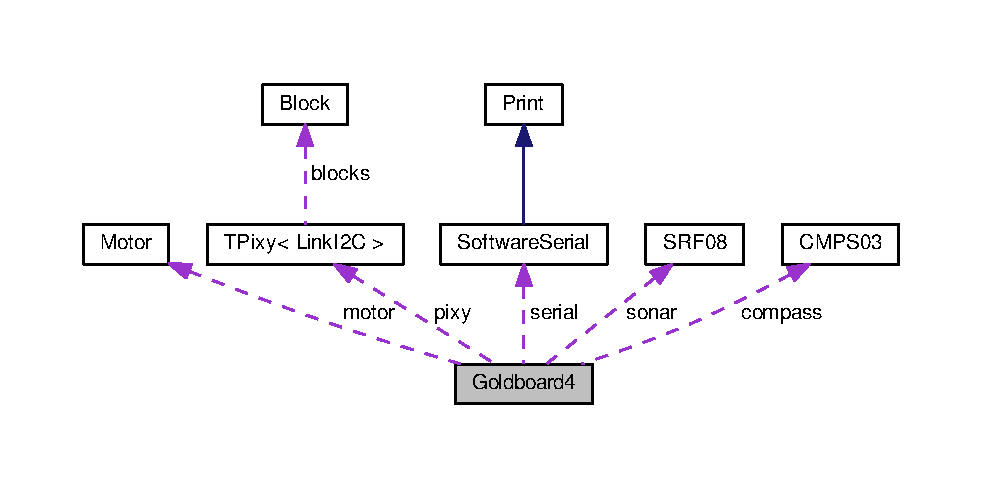
\includegraphics[width=350pt]{class_goldboard4__coll__graph}
\end{center}
\end{figure}
\subsection*{Public Member Functions}
\begin{DoxyCompactItemize}
\item 
void \hyperlink{class_goldboard4_a78c077cd2b846533cf1134f23dd2db79}{set\+Motors\+Off} ()
\item 
void \hyperlink{class_goldboard4_ac782bb10887e4cd6e58fcbe7b7d65623}{set\+Motors\+Offset} (int16\+\_\+t value)
\item 
void \hyperlink{class_goldboard4_a0c3134553d7136d32d46ea4641079c93}{init\+L\+ED} (uint8\+\_\+t i)
\item 
void \hyperlink{class_goldboard4_aedbe5a314f43d0da6dfed1bbb23b5ca2}{set\+Led} (uint8\+\_\+t i, bool state)
\item 
void \hyperlink{class_goldboard4_a09f18b8381af7830c2dc4214a6d84fbc}{set\+Power} (uint8\+\_\+t i, bool state)
\item 
void \hyperlink{class_goldboard4_a7fce81b6d0c23129da6e361badaefdf4}{set\+Power\+P\+WM} (uint8\+\_\+t i, uint8\+\_\+t state)
\item 
bool \hyperlink{class_goldboard4_aaf6ac85d732d07ffaa3ba88bed461a9a}{get\+Button} (uint8\+\_\+t i)
\item 
void \hyperlink{class_goldboard4_a2a83bb33f819b913fd63a95fe9a97bde}{wait\+For\+Button} (uint8\+\_\+t i)
\item 
uint8\+\_\+t \hyperlink{class_goldboard4_a81c498c9cfa45e7cc04883e561c24921}{get\+Analog} (uint8\+\_\+t i)
\item 
bool \hyperlink{class_goldboard4_a72afec46aecbca276d29e714ac5ab1b7}{get\+P\+WM} (uint8\+\_\+t i)
\item 
bool \hyperlink{class_goldboard4_a4fa6316d58b1e6b5b8174ee748b41216}{get\+Digital} (uint8\+\_\+t i)
\item 
void \hyperlink{class_goldboard4_a43c453224e2b6c04dbf040e82b419c50}{set\+P\+W\+M\+Servo} (uint8\+\_\+t value, uint8\+\_\+t pin)
\item 
void \hyperlink{class_goldboard4_afa78c637a7b8db1eae0eb8b3792f71e4}{reset\+P\+W\+M\+Servo} (uint8\+\_\+t pin)
\item 
void {\bfseries set\+Digital} (uint8\+\_\+t i, bool state)\hypertarget{class_goldboard4_a15872524d69b69fec2b00c63a90e5221}{}\label{class_goldboard4_a15872524d69b69fec2b00c63a90e5221}

\item 
uint8\+\_\+t \hyperlink{class_goldboard4_ac4f9d6eb4d800c68bffc065913427c73}{get\+Digital\+Pulsed\+Light} (uint8\+\_\+t i)
\item 
uint8\+\_\+t \hyperlink{class_goldboard4_abaedef75924a199b7779ce37028f11f8}{get\+P\+W\+M\+Pulsed\+Light} (uint8\+\_\+t i)
\item 
void {\bfseries scan\+I2C} ()\hypertarget{class_goldboard4_a7bb4ac08dc90ad14adb519a529519048}{}\label{class_goldboard4_a7bb4ac08dc90ad14adb519a529519048}

\end{DoxyCompactItemize}
\subsection*{Public Attributes}
\begin{DoxyCompactItemize}
\item 
\hyperlink{class_motor}{Motor} {\bfseries motor} \mbox{[}4\mbox{]}\hypertarget{class_goldboard4_ad4c496a805d72aa5c9dc89373c365c8d}{}\label{class_goldboard4_ad4c496a805d72aa5c9dc89373c365c8d}

\item 
\hyperlink{class_software_serial}{Software\+Serial} {\bfseries serial}\hypertarget{class_goldboard4_af133e9049fb5f1ade2de5402f209a0d0}{}\label{class_goldboard4_af133e9049fb5f1ade2de5402f209a0d0}

\item 
\hyperlink{class_c_m_p_s03}{C\+M\+P\+S03} {\bfseries compass}\hypertarget{class_goldboard4_abbe4d3f12b7003981f497ee200bfabd0}{}\label{class_goldboard4_abbe4d3f12b7003981f497ee200bfabd0}

\item 
\hyperlink{class_s_r_f08}{S\+R\+F08} {\bfseries sonar} \mbox{[}4\mbox{]}\hypertarget{class_goldboard4_ad33895d9300227e2ed714b6a43ade37f}{}\label{class_goldboard4_ad33895d9300227e2ed714b6a43ade37f}

\item 
\hyperlink{class_t_pixy}{Pixy\+I2C} {\bfseries pixy}\hypertarget{class_goldboard4_ad12ee511eff45283e6920cd8c82c7cc4}{}\label{class_goldboard4_ad12ee511eff45283e6920cd8c82c7cc4}

\item 
\hyperlink{classusring}{usring} {\bfseries bodensensor}\hypertarget{class_goldboard4_a13f2f620c8cdbc211e5651a114ddc912}{}\label{class_goldboard4_a13f2f620c8cdbc211e5651a114ddc912}

\item 
\hyperlink{class_v_l53_l0_x}{V\+L53\+L0X} {\bfseries Laser\+Sensor} \mbox{[}4\mbox{]}\hypertarget{class_goldboard4_a203effa1c5b0637b01c9d0e8685573dd}{}\label{class_goldboard4_a203effa1c5b0637b01c9d0e8685573dd}

\item 
\hyperlink{class_p_c_f8574_a}{P\+C\+F8574A} {\bfseries digital}\hypertarget{class_goldboard4_a01f0aa53885e0c2b59bbf5a424ec7588}{}\label{class_goldboard4_a01f0aa53885e0c2b59bbf5a424ec7588}

\end{DoxyCompactItemize}


\subsection{Member Function Documentation}
\index{Goldboard4@{Goldboard4}!get\+Analog@{get\+Analog}}
\index{get\+Analog@{get\+Analog}!Goldboard4@{Goldboard4}}
\subsubsection[{\texorpdfstring{get\+Analog(uint8\+\_\+t i)}{getAnalog(uint8_t i)}}]{\setlength{\rightskip}{0pt plus 5cm}uint8\+\_\+t Goldboard4\+::get\+Analog (
\begin{DoxyParamCaption}
\item[{uint8\+\_\+t}]{i}
\end{DoxyParamCaption}
)}\hypertarget{class_goldboard4_a81c498c9cfa45e7cc04883e561c24921}{}\label{class_goldboard4_a81c498c9cfa45e7cc04883e561c24921}
returns the value of the analog port i. 0 $<$= value $<$= 255 \index{Goldboard4@{Goldboard4}!get\+Button@{get\+Button}}
\index{get\+Button@{get\+Button}!Goldboard4@{Goldboard4}}
\subsubsection[{\texorpdfstring{get\+Button(uint8\+\_\+t i)}{getButton(uint8_t i)}}]{\setlength{\rightskip}{0pt plus 5cm}bool Goldboard4\+::get\+Button (
\begin{DoxyParamCaption}
\item[{uint8\+\_\+t}]{i}
\end{DoxyParamCaption}
)}\hypertarget{class_goldboard4_aaf6ac85d732d07ffaa3ba88bed461a9a}{}\label{class_goldboard4_aaf6ac85d732d07ffaa3ba88bed461a9a}
Checks the state of button i. If it is pressed, true is returned, else false. \index{Goldboard4@{Goldboard4}!get\+Digital@{get\+Digital}}
\index{get\+Digital@{get\+Digital}!Goldboard4@{Goldboard4}}
\subsubsection[{\texorpdfstring{get\+Digital(uint8\+\_\+t i)}{getDigital(uint8_t i)}}]{\setlength{\rightskip}{0pt plus 5cm}bool Goldboard4\+::get\+Digital (
\begin{DoxyParamCaption}
\item[{uint8\+\_\+t}]{i}
\end{DoxyParamCaption}
)}\hypertarget{class_goldboard4_a4fa6316d58b1e6b5b8174ee748b41216}{}\label{class_goldboard4_a4fa6316d58b1e6b5b8174ee748b41216}
returns true if the digital port is logical high, else false. \index{Goldboard4@{Goldboard4}!get\+Digital\+Pulsed\+Light@{get\+Digital\+Pulsed\+Light}}
\index{get\+Digital\+Pulsed\+Light@{get\+Digital\+Pulsed\+Light}!Goldboard4@{Goldboard4}}
\subsubsection[{\texorpdfstring{get\+Digital\+Pulsed\+Light(uint8\+\_\+t i)}{getDigitalPulsedLight(uint8_t i)}}]{\setlength{\rightskip}{0pt plus 5cm}uint8\+\_\+t Goldboard4\+::get\+Digital\+Pulsed\+Light (
\begin{DoxyParamCaption}
\item[{uint8\+\_\+t}]{i}
\end{DoxyParamCaption}
)}\hypertarget{class_goldboard4_ac4f9d6eb4d800c68bffc065913427c73}{}\label{class_goldboard4_ac4f9d6eb4d800c68bffc065913427c73}
returns the registered pulse length of the digital port i. 0 $<$= value $<$= 255 \index{Goldboard4@{Goldboard4}!get\+P\+WM@{get\+P\+WM}}
\index{get\+P\+WM@{get\+P\+WM}!Goldboard4@{Goldboard4}}
\subsubsection[{\texorpdfstring{get\+P\+W\+M(uint8\+\_\+t i)}{getPWM(uint8_t i)}}]{\setlength{\rightskip}{0pt plus 5cm}bool Goldboard4\+::get\+P\+WM (
\begin{DoxyParamCaption}
\item[{uint8\+\_\+t}]{i}
\end{DoxyParamCaption}
)}\hypertarget{class_goldboard4_a72afec46aecbca276d29e714ac5ab1b7}{}\label{class_goldboard4_a72afec46aecbca276d29e714ac5ab1b7}
returns true if the pwm port is logical high, else false. \index{Goldboard4@{Goldboard4}!get\+P\+W\+M\+Pulsed\+Light@{get\+P\+W\+M\+Pulsed\+Light}}
\index{get\+P\+W\+M\+Pulsed\+Light@{get\+P\+W\+M\+Pulsed\+Light}!Goldboard4@{Goldboard4}}
\subsubsection[{\texorpdfstring{get\+P\+W\+M\+Pulsed\+Light(uint8\+\_\+t i)}{getPWMPulsedLight(uint8_t i)}}]{\setlength{\rightskip}{0pt plus 5cm}uint8\+\_\+t Goldboard4\+::get\+P\+W\+M\+Pulsed\+Light (
\begin{DoxyParamCaption}
\item[{uint8\+\_\+t}]{i}
\end{DoxyParamCaption}
)}\hypertarget{class_goldboard4_abaedef75924a199b7779ce37028f11f8}{}\label{class_goldboard4_abaedef75924a199b7779ce37028f11f8}
returns the registered pulse length of the pwm port i. 0 $<$= value $<$= 255

returns the registered pulse length of the digital port i. 0 $<$= value $<$= 255 \index{Goldboard4@{Goldboard4}!init\+L\+ED@{init\+L\+ED}}
\index{init\+L\+ED@{init\+L\+ED}!Goldboard4@{Goldboard4}}
\subsubsection[{\texorpdfstring{init\+L\+E\+D(uint8\+\_\+t i)}{initLED(uint8_t i)}}]{\setlength{\rightskip}{0pt plus 5cm}void Goldboard4\+::init\+L\+ED (
\begin{DoxyParamCaption}
\item[{uint8\+\_\+t}]{i}
\end{DoxyParamCaption}
)}\hypertarget{class_goldboard4_a0c3134553d7136d32d46ea4641079c93}{}\label{class_goldboard4_a0c3134553d7136d32d46ea4641079c93}
sets the given led id as led (N\+O\+TE\+: Then this pin cannot be used as button anymore) \index{Goldboard4@{Goldboard4}!reset\+P\+W\+M\+Servo@{reset\+P\+W\+M\+Servo}}
\index{reset\+P\+W\+M\+Servo@{reset\+P\+W\+M\+Servo}!Goldboard4@{Goldboard4}}
\subsubsection[{\texorpdfstring{reset\+P\+W\+M\+Servo(uint8\+\_\+t pin)}{resetPWMServo(uint8_t pin)}}]{\setlength{\rightskip}{0pt plus 5cm}void Goldboard4\+::reset\+P\+W\+M\+Servo (
\begin{DoxyParamCaption}
\item[{uint8\+\_\+t}]{pin}
\end{DoxyParamCaption}
)}\hypertarget{class_goldboard4_afa78c637a7b8db1eae0eb8b3792f71e4}{}\label{class_goldboard4_afa78c637a7b8db1eae0eb8b3792f71e4}
don\textquotesingle{}t use this function to stop your brushless motor. Use set\+P\+W\+M\+Servo(i,0) instead

stops the P\+WM pulse. Dont use this, if you want to stop a brushless motor. Use set\+P\+W\+M\+Servo(0,0) instead. \index{Goldboard4@{Goldboard4}!set\+Led@{set\+Led}}
\index{set\+Led@{set\+Led}!Goldboard4@{Goldboard4}}
\subsubsection[{\texorpdfstring{set\+Led(uint8\+\_\+t i, bool state)}{setLed(uint8_t i, bool state)}}]{\setlength{\rightskip}{0pt plus 5cm}void Goldboard4\+::set\+Led (
\begin{DoxyParamCaption}
\item[{uint8\+\_\+t}]{i, }
\item[{bool}]{state}
\end{DoxyParamCaption}
)}\hypertarget{class_goldboard4_aedbe5a314f43d0da6dfed1bbb23b5ca2}{}\label{class_goldboard4_aedbe5a314f43d0da6dfed1bbb23b5ca2}
Puts L\+ED i on if state is true, else off \index{Goldboard4@{Goldboard4}!set\+Motors\+Off@{set\+Motors\+Off}}
\index{set\+Motors\+Off@{set\+Motors\+Off}!Goldboard4@{Goldboard4}}
\subsubsection[{\texorpdfstring{set\+Motors\+Off()}{setMotorsOff()}}]{\setlength{\rightskip}{0pt plus 5cm}void Goldboard4\+::set\+Motors\+Off (
\begin{DoxyParamCaption}
{}
\end{DoxyParamCaption}
)}\hypertarget{class_goldboard4_a78c077cd2b846533cf1134f23dd2db79}{}\label{class_goldboard4_a78c077cd2b846533cf1134f23dd2db79}
Puts off all motors. \index{Goldboard4@{Goldboard4}!set\+Motors\+Offset@{set\+Motors\+Offset}}
\index{set\+Motors\+Offset@{set\+Motors\+Offset}!Goldboard4@{Goldboard4}}
\subsubsection[{\texorpdfstring{set\+Motors\+Offset(int16\+\_\+t value)}{setMotorsOffset(int16_t value)}}]{\setlength{\rightskip}{0pt plus 5cm}void Goldboard4\+::set\+Motors\+Offset (
\begin{DoxyParamCaption}
\item[{int16\+\_\+t}]{val}
\end{DoxyParamCaption}
)}\hypertarget{class_goldboard4_ac782bb10887e4cd6e58fcbe7b7d65623}{}\label{class_goldboard4_ac782bb10887e4cd6e58fcbe7b7d65623}
Sets a motor offset \index{Goldboard4@{Goldboard4}!set\+Power@{set\+Power}}
\index{set\+Power@{set\+Power}!Goldboard4@{Goldboard4}}
\subsubsection[{\texorpdfstring{set\+Power(uint8\+\_\+t i, bool state)}{setPower(uint8_t i, bool state)}}]{\setlength{\rightskip}{0pt plus 5cm}void Goldboard4\+::set\+Power (
\begin{DoxyParamCaption}
\item[{uint8\+\_\+t}]{i, }
\item[{bool}]{state}
\end{DoxyParamCaption}
)}\hypertarget{class_goldboard4_a09f18b8381af7830c2dc4214a6d84fbc}{}\label{class_goldboard4_a09f18b8381af7830c2dc4214a6d84fbc}
Puts the power output i on if state is true, else off \index{Goldboard4@{Goldboard4}!set\+Power\+P\+WM@{set\+Power\+P\+WM}}
\index{set\+Power\+P\+WM@{set\+Power\+P\+WM}!Goldboard4@{Goldboard4}}
\subsubsection[{\texorpdfstring{set\+Power\+P\+W\+M(uint8\+\_\+t i, uint8\+\_\+t state)}{setPowerPWM(uint8_t i, uint8_t state)}}]{\setlength{\rightskip}{0pt plus 5cm}void Goldboard4\+::set\+Power\+P\+WM (
\begin{DoxyParamCaption}
\item[{uint8\+\_\+t}]{i, }
\item[{uint8\+\_\+t}]{state}
\end{DoxyParamCaption}
)}\hypertarget{class_goldboard4_a7fce81b6d0c23129da6e361badaefdf4}{}\label{class_goldboard4_a7fce81b6d0c23129da6e361badaefdf4}
Puts the power i in P\+WM mode. state is a value from 0 -\/ 255. \index{Goldboard4@{Goldboard4}!set\+P\+W\+M\+Servo@{set\+P\+W\+M\+Servo}}
\index{set\+P\+W\+M\+Servo@{set\+P\+W\+M\+Servo}!Goldboard4@{Goldboard4}}
\subsubsection[{\texorpdfstring{set\+P\+W\+M\+Servo(uint8\+\_\+t value, uint8\+\_\+t pin)}{setPWMServo(uint8_t value, uint8_t pin)}}]{\setlength{\rightskip}{0pt plus 5cm}void Goldboard4\+::set\+P\+W\+M\+Servo (
\begin{DoxyParamCaption}
\item[{uint8\+\_\+t}]{value, }
\item[{uint8\+\_\+t}]{pin}
\end{DoxyParamCaption}
)}\hypertarget{class_goldboard4_a43c453224e2b6c04dbf040e82b419c50}{}\label{class_goldboard4_a43c453224e2b6c04dbf040e82b419c50}
sets the P\+WM pin (0-\/7) as Servo Output and sends a certain value (0-\/255) every 20 ms

sets the P\+WM pin (0-\/7) as Servo Output and sends a certain value (0-\/255 $\sim$ 0.\+8-\/2.\+8ms pulse) every 20 ms \index{Goldboard4@{Goldboard4}!wait\+For\+Button@{wait\+For\+Button}}
\index{wait\+For\+Button@{wait\+For\+Button}!Goldboard4@{Goldboard4}}
\subsubsection[{\texorpdfstring{wait\+For\+Button(uint8\+\_\+t i)}{waitForButton(uint8_t i)}}]{\setlength{\rightskip}{0pt plus 5cm}void Goldboard4\+::wait\+For\+Button (
\begin{DoxyParamCaption}
\item[{uint8\+\_\+t}]{i}
\end{DoxyParamCaption}
)}\hypertarget{class_goldboard4_a2a83bb33f819b913fd63a95fe9a97bde}{}\label{class_goldboard4_a2a83bb33f819b913fd63a95fe9a97bde}
Waits until button i is pressed and released again. 

The documentation for this class was generated from the following files\+:\begin{DoxyCompactItemize}
\item 
/home/alex/workspace/goldboard4/libs/goldboard4/Goldboard4.\+h\item 
/home/alex/workspace/goldboard4/libs/goldboard4/Goldboard4.\+cpp\end{DoxyCompactItemize}

\hypertarget{class_h_c05}{}\section{H\+C05 Class Reference}
\label{class_h_c05}\index{H\+C05@{H\+C05}}
\subsection*{Public Member Functions}
\begin{DoxyCompactItemize}
\item 
{\bfseries H\+C05} (const char $\ast$device\+Name, const char $\ast$Password)\hypertarget{class_h_c05_a16354dfb5fb4aecd0e46f6b1e52bba19}{}\label{class_h_c05_a16354dfb5fb4aecd0e46f6b1e52bba19}

\item 
uint8\+\_\+t \hyperlink{class_h_c05_aa898f70439bdfa3f1ee0aba70bd6e236}{set\+Pairing\+Password} (const char $\ast$Password)
\item 
uint8\+\_\+t {\bfseries set\+Device\+Name} (const char $\ast$device\+Name)\hypertarget{class_h_c05_a4cf49a9ae47ab51d4dcc62c7e930665c}{}\label{class_h_c05_a4cf49a9ae47ab51d4dcc62c7e930665c}

\item 
uint8\+\_\+t {\bfseries pair\+With} (const char $\ast$device\+Name, const char $\ast$Password)\hypertarget{class_h_c05_a90cfb4e5b0d784dc419d93e317bffc72}{}\label{class_h_c05_a90cfb4e5b0d784dc419d93e317bffc72}

\item 
uint8\+\_\+t {\bfseries inquier\+Pairing} ()\hypertarget{class_h_c05_ad649d18c9a925a65d26ffe7f5c668df5}{}\label{class_h_c05_ad649d18c9a925a65d26ffe7f5c668df5}

\item 
uint8\+\_\+t {\bfseries inquier\+Pairing} (int timeout)\hypertarget{class_h_c05_a714e778e6eb2ed8852dc9cf38788b600}{}\label{class_h_c05_a714e778e6eb2ed8852dc9cf38788b600}

\item 
bool {\bfseries is\+Connected} ()\hypertarget{class_h_c05_adf8eba3cca2adc175fc2fc67fb226aa1}{}\label{class_h_c05_adf8eba3cca2adc175fc2fc67fb226aa1}

\item 
bool {\bfseries send\+Byte} (uint8\+\_\+t byte)\hypertarget{class_h_c05_a4ab3baf3969a57260abf0aead48eefd9}{}\label{class_h_c05_a4ab3baf3969a57260abf0aead48eefd9}

\item 
bool {\bfseries send\+String} (const char $\ast$data)\hypertarget{class_h_c05_a350d418bd42b13c8b71e9ee535513de4}{}\label{class_h_c05_a350d418bd42b13c8b71e9ee535513de4}

\item 
int {\bfseries get\+Line} (char $\ast$buffer, int buffersize)\hypertarget{class_h_c05_a60becf23b1660d5f3a70d8e595c23d65}{}\label{class_h_c05_a60becf23b1660d5f3a70d8e595c23d65}

\item 
uint8\+\_\+t {\bfseries factory\+Reset\+Device} ()\hypertarget{class_h_c05_ace697b72e9f49a9426c1c4c4690a7c2b}{}\label{class_h_c05_ace697b72e9f49a9426c1c4c4690a7c2b}

\item 
uint8\+\_\+t {\bfseries reset\+Device} ()\hypertarget{class_h_c05_aeaf0e5a706c38668d5c6e1e3a2da9530}{}\label{class_h_c05_aeaf0e5a706c38668d5c6e1e3a2da9530}

\item 
uint8\+\_\+t {\bfseries get\+Status} ()\hypertarget{class_h_c05_a8c3253de07a3bfbba160c8d3d445ca1a}{}\label{class_h_c05_a8c3253de07a3bfbba160c8d3d445ca1a}

\item 
bool {\bfseries init} ()\hypertarget{class_h_c05_acd0883af068fac1ea46aa2efbd901916}{}\label{class_h_c05_acd0883af068fac1ea46aa2efbd901916}

\item 
uint8\+\_\+t {\bfseries getlast\+Error} ()\hypertarget{class_h_c05_a42e12cca5c4ad4c198dcc31eb7f78e29}{}\label{class_h_c05_a42e12cca5c4ad4c198dcc31eb7f78e29}

\item 
uint8\+\_\+t {\bfseries set\+Mode} (const char $\ast$mode)\hypertarget{class_h_c05_a9351e5325cdca07ffb03f80939cc843a}{}\label{class_h_c05_a9351e5325cdca07ffb03f80939cc843a}

\end{DoxyCompactItemize}


\subsection{Member Function Documentation}
\index{H\+C05@{H\+C05}!set\+Pairing\+Password@{set\+Pairing\+Password}}
\index{set\+Pairing\+Password@{set\+Pairing\+Password}!H\+C05@{H\+C05}}
\subsubsection[{\texorpdfstring{set\+Pairing\+Password(const char $\ast$\+Password)}{setPairingPassword(const char *Password)}}]{\setlength{\rightskip}{0pt plus 5cm}uint8\+\_\+t H\+C05\+::set\+Pairing\+Password (
\begin{DoxyParamCaption}
\item[{const char $\ast$}]{Password}
\end{DoxyParamCaption}
)}\hypertarget{class_h_c05_aa898f70439bdfa3f1ee0aba70bd6e236}{}\label{class_h_c05_aa898f70439bdfa3f1ee0aba70bd6e236}
configuration 

The documentation for this class was generated from the following files\+:\begin{DoxyCompactItemize}
\item 
/home/alex/workspace/goldboard4/goldboard/H\+C05.\+h\item 
/home/alex/workspace/goldboard4/goldboard/H\+C05.\+cpp\end{DoxyCompactItemize}

\hypertarget{class_link_i2_c}{}\section{Link\+I2C Class Reference}
\label{class_link_i2_c}\index{Link\+I2C@{Link\+I2C}}
\subsection*{Public Member Functions}
\begin{DoxyCompactItemize}
\item 
void {\bfseries init} ()\hypertarget{class_link_i2_c_a88bb723d5558bdc9011d383ec6ead785}{}\label{class_link_i2_c_a88bb723d5558bdc9011d383ec6ead785}

\item 
void {\bfseries set\+Arg} (uint16\+\_\+t arg)\hypertarget{class_link_i2_c_a5f15394cf091ad6f209a64cf0f0db7ae}{}\label{class_link_i2_c_a5f15394cf091ad6f209a64cf0f0db7ae}

\item 
uint16\+\_\+t {\bfseries get\+Word} ()\hypertarget{class_link_i2_c_a7f0d784f6aea082e92392b86aa26e137}{}\label{class_link_i2_c_a7f0d784f6aea082e92392b86aa26e137}

\item 
uint8\+\_\+t {\bfseries get\+Byte} ()\hypertarget{class_link_i2_c_a13520ec81c6b8d2fb5dd443b35cbb778}{}\label{class_link_i2_c_a13520ec81c6b8d2fb5dd443b35cbb778}

\item 
int8\+\_\+t {\bfseries send} (uint8\+\_\+t $\ast$data, uint8\+\_\+t len)\hypertarget{class_link_i2_c_ae7b12321ba087e83fe265ede5e84bc07}{}\label{class_link_i2_c_ae7b12321ba087e83fe265ede5e84bc07}

\end{DoxyCompactItemize}


The documentation for this class was generated from the following file\+:\begin{DoxyCompactItemize}
\item 
/home/alex/workspace/goldboard4/goldboard/Pixy\+I2\+C.\+h\end{DoxyCompactItemize}

\hypertarget{class_link_u_a_r_t}{}\section{Link\+U\+A\+RT Class Reference}
\label{class_link_u_a_r_t}\index{Link\+U\+A\+RT@{Link\+U\+A\+RT}}
\subsection*{Public Member Functions}
\begin{DoxyCompactItemize}
\item 
void {\bfseries init} ()\hypertarget{class_link_u_a_r_t_a01a9c561421f4ddb04f329219eb2e100}{}\label{class_link_u_a_r_t_a01a9c561421f4ddb04f329219eb2e100}

\item 
void {\bfseries set\+Arg} (uint16\+\_\+t arg)\hypertarget{class_link_u_a_r_t_a26a7fe9330f846de273637517a0f092c}{}\label{class_link_u_a_r_t_a26a7fe9330f846de273637517a0f092c}

\item 
uint16\+\_\+t {\bfseries get\+Word} ()\hypertarget{class_link_u_a_r_t_af8d40edd838c32f455cd64a9399e1279}{}\label{class_link_u_a_r_t_af8d40edd838c32f455cd64a9399e1279}

\item 
uint8\+\_\+t {\bfseries get\+Byte} ()\hypertarget{class_link_u_a_r_t_aeead28b04db5dd81516af99125b74f30}{}\label{class_link_u_a_r_t_aeead28b04db5dd81516af99125b74f30}

\item 
int8\+\_\+t {\bfseries send} (uint8\+\_\+t $\ast$data, uint8\+\_\+t len)\hypertarget{class_link_u_a_r_t_ae39f94886b5656fcd391be7e3d26f6b5}{}\label{class_link_u_a_r_t_ae39f94886b5656fcd391be7e3d26f6b5}

\end{DoxyCompactItemize}


The documentation for this class was generated from the following file\+:\begin{DoxyCompactItemize}
\item 
/home/alex/workspace/goldboard4/libs/goldboard4/Pixy\+U\+A\+R\+T.\+h\end{DoxyCompactItemize}

\hypertarget{class_motor}{}\section{Motor Class Reference}
\label{class_motor}\index{Motor@{Motor}}
\subsection*{Public Member Functions}
\begin{DoxyCompactItemize}
\item 
void {\bfseries init} (uint8\+\_\+t direction\+Pin\+First, uint8\+\_\+t direction\+Pin\+Second, uint8\+\_\+t speed\+Pin, \hyperlink{class_p_c_f8574_a}{P\+C\+F8574A} $\ast$, uint8\+\_\+t $\ast$)\hypertarget{class_motor_a9bfe106b0b35300d4c50bdb996a6d75c}{}\label{class_motor_a9bfe106b0b35300d4c50bdb996a6d75c}

\item 
void {\bfseries rotate} (int16\+\_\+t speed)\hypertarget{class_motor_aa5088f286e723e55cc38fe712e847c63}{}\label{class_motor_aa5088f286e723e55cc38fe712e847c63}

\item 
void {\bfseries stop} (bool bremsen)\hypertarget{class_motor_ab0b38acc90da22cbeb5f4b0234616e52}{}\label{class_motor_ab0b38acc90da22cbeb5f4b0234616e52}

\item 
void {\bfseries acceleration\+Handler} ()\hypertarget{class_motor_a71e53d91b88aa532c4ae8bccac3a85ad}{}\label{class_motor_a71e53d91b88aa532c4ae8bccac3a85ad}

\item 
void {\bfseries rotate\+Direct} (int16\+\_\+t speed)\hypertarget{class_motor_a8f9a423dd18e005b2e732324031730bb}{}\label{class_motor_a8f9a423dd18e005b2e732324031730bb}

\item 
void {\bfseries set\+Acceleration} (uint8\+\_\+t percent\+Per\+Hundret\+Ms)\hypertarget{class_motor_ae5d7052859ad6cff34184a6794af4222}{}\label{class_motor_ae5d7052859ad6cff34184a6794af4222}

\end{DoxyCompactItemize}
\subsection*{Public Attributes}
\begin{DoxyCompactItemize}
\item 
uint8\+\_\+t $\ast$ {\bfseries speed}\hypertarget{class_motor_a1dbc9bc30ae5271f34b31c8d0ea59d0b}{}\label{class_motor_a1dbc9bc30ae5271f34b31c8d0ea59d0b}

\end{DoxyCompactItemize}


The documentation for this class was generated from the following files\+:\begin{DoxyCompactItemize}
\item 
/home/alex/workspace/goldboard4/libs/goldboard4/Motor.\+h\item 
/home/alex/workspace/goldboard4/libs/goldboard4/Motor.\+cpp\end{DoxyCompactItemize}

\hypertarget{struct_stream_1_1_multi_target}{}\section{Stream\+:\+:Multi\+Target Struct Reference}
\label{struct_stream_1_1_multi_target}\index{Stream\+::\+Multi\+Target@{Stream\+::\+Multi\+Target}}
\subsection*{Public Attributes}
\begin{DoxyCompactItemize}
\item 
const char $\ast$ {\bfseries str}\hypertarget{struct_stream_1_1_multi_target_a2966d33f06cd1f5db43702f08c6e74c7}{}\label{struct_stream_1_1_multi_target_a2966d33f06cd1f5db43702f08c6e74c7}

\item 
size\+\_\+t {\bfseries len}\hypertarget{struct_stream_1_1_multi_target_ae0ffba42be1143525f624242bf607a63}{}\label{struct_stream_1_1_multi_target_ae0ffba42be1143525f624242bf607a63}

\item 
size\+\_\+t {\bfseries index}\hypertarget{struct_stream_1_1_multi_target_a33cced896eb2dbabbeb7dd5dfa019e51}{}\label{struct_stream_1_1_multi_target_a33cced896eb2dbabbeb7dd5dfa019e51}

\end{DoxyCompactItemize}


The documentation for this struct was generated from the following file\+:\begin{DoxyCompactItemize}
\item 
/home/alex/workspace/goldboard4/libs/goldboard4/Stream.\+h\end{DoxyCompactItemize}

\hypertarget{class_p_c_f8574_a}{}\section{P\+C\+F8574A Class Reference}
\label{class_p_c_f8574_a}\index{P\+C\+F8574A@{P\+C\+F8574A}}
\subsection*{Public Member Functions}
\begin{DoxyCompactItemize}
\item 
void {\bfseries set\+Pin} (uint8\+\_\+t, bool)\hypertarget{class_p_c_f8574_a_a8612893eb323b38c8c31fb1e415b9eff}{}\label{class_p_c_f8574_a_a8612893eb323b38c8c31fb1e415b9eff}

\item 
uint8\+\_\+t {\bfseries read} ()\hypertarget{class_p_c_f8574_a_ab8bbb865bc98e8f4c2fdc5b30d81df43}{}\label{class_p_c_f8574_a_ab8bbb865bc98e8f4c2fdc5b30d81df43}

\item 
void {\bfseries write} ()\hypertarget{class_p_c_f8574_a_ab462fef7ab449d66c921913c7b5608e4}{}\label{class_p_c_f8574_a_ab462fef7ab449d66c921913c7b5608e4}

\end{DoxyCompactItemize}


The documentation for this class was generated from the following files\+:\begin{DoxyCompactItemize}
\item 
/home/alex/workspace/goldboard4/goldboard/P\+C\+F8574\+A.\+h\item 
/home/alex/workspace/goldboard4/goldboard/P\+C\+F8574\+A.\+cpp\end{DoxyCompactItemize}

\hypertarget{class_print}{}\section{Print Class Reference}
\label{class_print}\index{Print@{Print}}


Inheritance diagram for Print\+:
\nopagebreak
\begin{figure}[H]
\begin{center}
\leavevmode
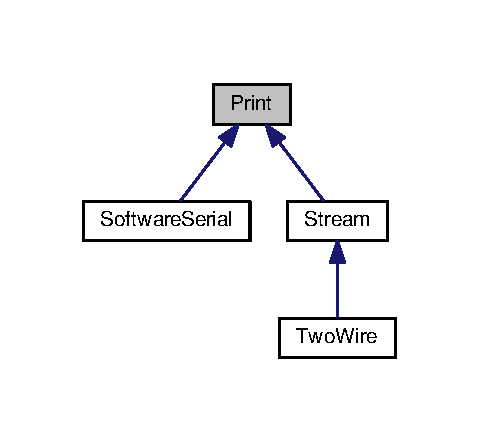
\includegraphics[width=230pt]{class_print__inherit__graph}
\end{center}
\end{figure}
\subsection*{Public Member Functions}
\begin{DoxyCompactItemize}
\item 
int {\bfseries get\+Write\+Error} ()\hypertarget{class_print_a88a4a829fb5d589efb43955ad0cbddcc}{}\label{class_print_a88a4a829fb5d589efb43955ad0cbddcc}

\item 
void {\bfseries clear\+Write\+Error} ()\hypertarget{class_print_aec9ecf84cc6d9087a650def3cefc459e}{}\label{class_print_aec9ecf84cc6d9087a650def3cefc459e}

\item 
virtual size\+\_\+t {\bfseries write} (uint8\+\_\+t)=0\hypertarget{class_print_a5be30d49adae2406a270c29ba9a3e0a3}{}\label{class_print_a5be30d49adae2406a270c29ba9a3e0a3}

\item 
size\+\_\+t {\bfseries write} (const char $\ast$str)\hypertarget{class_print_a5b40e0e9cab1f2fe5bb0cb22ffe5adda}{}\label{class_print_a5b40e0e9cab1f2fe5bb0cb22ffe5adda}

\item 
virtual size\+\_\+t {\bfseries write} (const uint8\+\_\+t $\ast$buffer, size\+\_\+t size)\hypertarget{class_print_ad98d820df11e2697be1e4b1ea30b4a23}{}\label{class_print_ad98d820df11e2697be1e4b1ea30b4a23}

\item 
size\+\_\+t {\bfseries write} (const char $\ast$buffer, size\+\_\+t size)\hypertarget{class_print_abfdd93a61c4b95a3ba41680188505e73}{}\label{class_print_abfdd93a61c4b95a3ba41680188505e73}

\item 
size\+\_\+t {\bfseries print} (const \+\_\+\+\_\+\+Flash\+String\+Helper $\ast$)\hypertarget{class_print_aa4158dd94bc1741f92d99c427261d7c0}{}\label{class_print_aa4158dd94bc1741f92d99c427261d7c0}

\item 
size\+\_\+t {\bfseries print} (const String \&)\hypertarget{class_print_a157007ca7ea8334ba7eb4bc705740216}{}\label{class_print_a157007ca7ea8334ba7eb4bc705740216}

\item 
size\+\_\+t {\bfseries print} (const char\mbox{[}$\,$\mbox{]})\hypertarget{class_print_acfe80773011eb17dfb52c2fba517a093}{}\label{class_print_acfe80773011eb17dfb52c2fba517a093}

\item 
size\+\_\+t {\bfseries print} (char)\hypertarget{class_print_a1e411d07a8ffec5faf7ce485bac0f029}{}\label{class_print_a1e411d07a8ffec5faf7ce485bac0f029}

\item 
size\+\_\+t {\bfseries print} (unsigned char, int=D\+EC)\hypertarget{class_print_a97bd44df9222fa4a51a1266fab8d3bc1}{}\label{class_print_a97bd44df9222fa4a51a1266fab8d3bc1}

\item 
size\+\_\+t {\bfseries print} (int, int=D\+EC)\hypertarget{class_print_a32cb3cf32d701c797b2b2d1080052dfe}{}\label{class_print_a32cb3cf32d701c797b2b2d1080052dfe}

\item 
size\+\_\+t {\bfseries print} (unsigned int, int=D\+EC)\hypertarget{class_print_a87275de35583868a370f43ce1c887750}{}\label{class_print_a87275de35583868a370f43ce1c887750}

\item 
size\+\_\+t {\bfseries print} (long, int=D\+EC)\hypertarget{class_print_ab1fb2a2384c7b9f628943f5046e7d1c1}{}\label{class_print_ab1fb2a2384c7b9f628943f5046e7d1c1}

\item 
size\+\_\+t {\bfseries print} (unsigned long, int=D\+EC)\hypertarget{class_print_a26a40be7a557c0bc391a15dce9f06954}{}\label{class_print_a26a40be7a557c0bc391a15dce9f06954}

\item 
size\+\_\+t {\bfseries print} (double, int=2)\hypertarget{class_print_ae8b4c025786c820afe0a90aeea01c9c5}{}\label{class_print_ae8b4c025786c820afe0a90aeea01c9c5}

\item 
size\+\_\+t {\bfseries print} (const \hyperlink{class_printable}{Printable} \&)\hypertarget{class_print_a901b0f06ae34aab31b8fbb4298f0596e}{}\label{class_print_a901b0f06ae34aab31b8fbb4298f0596e}

\item 
size\+\_\+t {\bfseries println} (const \+\_\+\+\_\+\+Flash\+String\+Helper $\ast$)\hypertarget{class_print_a4fd286b325d3b1a786cfa35072a8ef52}{}\label{class_print_a4fd286b325d3b1a786cfa35072a8ef52}

\item 
size\+\_\+t {\bfseries println} (const String \&s)\hypertarget{class_print_afd6cc6e2c1163f94c60855ad233899bd}{}\label{class_print_afd6cc6e2c1163f94c60855ad233899bd}

\item 
size\+\_\+t {\bfseries println} (const char\mbox{[}$\,$\mbox{]})\hypertarget{class_print_ad337ce3f7977411b7d34d47a51e5737e}{}\label{class_print_ad337ce3f7977411b7d34d47a51e5737e}

\item 
size\+\_\+t {\bfseries println} (char)\hypertarget{class_print_a554896a71162f967b5794401239d7a01}{}\label{class_print_a554896a71162f967b5794401239d7a01}

\item 
size\+\_\+t {\bfseries println} (unsigned char, int=D\+EC)\hypertarget{class_print_ac9afe80f50f0118d735295aec7727e50}{}\label{class_print_ac9afe80f50f0118d735295aec7727e50}

\item 
size\+\_\+t {\bfseries println} (int, int=D\+EC)\hypertarget{class_print_a738c88471cfb8eac7c8a804699971413}{}\label{class_print_a738c88471cfb8eac7c8a804699971413}

\item 
size\+\_\+t {\bfseries println} (unsigned int, int=D\+EC)\hypertarget{class_print_ac87eed1fcb78641169ba2244278c899e}{}\label{class_print_ac87eed1fcb78641169ba2244278c899e}

\item 
size\+\_\+t {\bfseries println} (long, int=D\+EC)\hypertarget{class_print_a833fbec3ceba92e3ec95f51e026e4569}{}\label{class_print_a833fbec3ceba92e3ec95f51e026e4569}

\item 
size\+\_\+t {\bfseries println} (unsigned long, int=D\+EC)\hypertarget{class_print_aebee3c33ee5d8f10b6f378d5273742d0}{}\label{class_print_aebee3c33ee5d8f10b6f378d5273742d0}

\item 
size\+\_\+t {\bfseries println} (double, int=2)\hypertarget{class_print_a56e976b079361b6021ef7c2bedb397a2}{}\label{class_print_a56e976b079361b6021ef7c2bedb397a2}

\item 
size\+\_\+t {\bfseries println} (const \hyperlink{class_printable}{Printable} \&)\hypertarget{class_print_a20f9e104153b62e720c9b4c348b44f00}{}\label{class_print_a20f9e104153b62e720c9b4c348b44f00}

\item 
size\+\_\+t {\bfseries println} (void)\hypertarget{class_print_a169b128f9e22f0c15883768f580541a2}{}\label{class_print_a169b128f9e22f0c15883768f580541a2}

\end{DoxyCompactItemize}
\subsection*{Protected Member Functions}
\begin{DoxyCompactItemize}
\item 
void {\bfseries set\+Write\+Error} (int err=1)\hypertarget{class_print_a46656410e23c0ec14d7a01b38b3b6f00}{}\label{class_print_a46656410e23c0ec14d7a01b38b3b6f00}

\end{DoxyCompactItemize}


The documentation for this class was generated from the following files\+:\begin{DoxyCompactItemize}
\item 
/home/alex/workspace/goldboard4/goldboard/Print.\+h\item 
/home/alex/workspace/goldboard4/goldboard/Print.\+cpp\end{DoxyCompactItemize}

\hypertarget{class_printable}{}\section{Printable Class Reference}
\label{class_printable}\index{Printable@{Printable}}


{\ttfamily \#include $<$Printable.\+h$>$}

\subsection*{Public Member Functions}
\begin{DoxyCompactItemize}
\item 
virtual size\+\_\+t {\bfseries print\+To} (\hyperlink{class_print}{Print} \&p) const =0\hypertarget{class_printable_a2c5776bc55c0a3a5675bba9d4d8e3681}{}\label{class_printable_a2c5776bc55c0a3a5675bba9d4d8e3681}

\end{DoxyCompactItemize}


\subsection{Detailed Description}
The \hyperlink{class_printable}{Printable} class provides a way for new classes to allow themselves to be printed. By deriving from \hyperlink{class_printable}{Printable} and implementing the print\+To method, it will then be possible for users to print out instances of this class by passing them into the usual Print\+::print and Print\+::println methods. 

The documentation for this class was generated from the following file\+:\begin{DoxyCompactItemize}
\item 
/home/alex/workspace/goldboard4/libs/goldboard4/Printable.\+h\end{DoxyCompactItemize}

\hypertarget{class_software_serial}{}\section{Software\+Serial Class Reference}
\label{class_software_serial}\index{Software\+Serial@{Software\+Serial}}


Inheritance diagram for Software\+Serial\+:\nopagebreak
\begin{figure}[H]
\begin{center}
\leavevmode
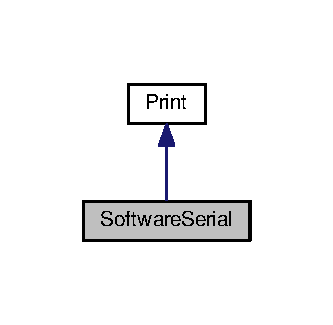
\includegraphics[width=160pt]{class_software_serial__inherit__graph}
\end{center}
\end{figure}


Collaboration diagram for Software\+Serial\+:\nopagebreak
\begin{figure}[H]
\begin{center}
\leavevmode
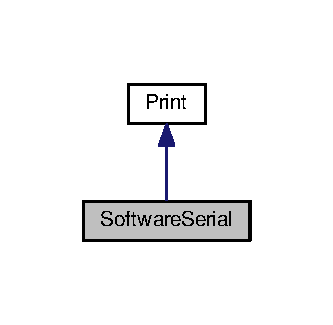
\includegraphics[width=160pt]{class_software_serial__coll__graph}
\end{center}
\end{figure}
\subsection*{Public Member Functions}
\begin{DoxyCompactItemize}
\item 
void {\bfseries begin} (unsigned long)\hypertarget{class_software_serial_a2c080b19d958967689c3fad7b6620844}{}\label{class_software_serial_a2c080b19d958967689c3fad7b6620844}

\item 
virtual size\+\_\+t {\bfseries write} (uint8\+\_\+t)\hypertarget{class_software_serial_a1481a56fb169a6529af6277bd87d39ac}{}\label{class_software_serial_a1481a56fb169a6529af6277bd87d39ac}

\end{DoxyCompactItemize}
\subsection*{Additional Inherited Members}


The documentation for this class was generated from the following files\+:\begin{DoxyCompactItemize}
\item 
/home/alex/workspace/goldboard4/libs/goldboard4/Serial.\+h\item 
/home/alex/workspace/goldboard4/libs/goldboard4/Serial.\+cpp\end{DoxyCompactItemize}

\hypertarget{class_s_r_f08}{}\section{S\+R\+F08 Class Reference}
\label{class_s_r_f08}\index{S\+R\+F08@{S\+R\+F08}}
\subsection*{Public Member Functions}
\begin{DoxyCompactItemize}
\item 
void {\bfseries init} (uint8\+\_\+t address)\hypertarget{class_s_r_f08_a2f2920aeafb6916589c1a9a7f2443dc6}{}\label{class_s_r_f08_a2f2920aeafb6916589c1a9a7f2443dc6}

\item 
void {\bfseries change\+Address} (uint8\+\_\+t new\+Address)\hypertarget{class_s_r_f08_a3b94c05d2c9aa0bbdde496f637875a4c}{}\label{class_s_r_f08_a3b94c05d2c9aa0bbdde496f637875a4c}

\item 
int {\bfseries get\+Value\+CM} ()\hypertarget{class_s_r_f08_abe78d5649f8bade345a5e42cd6bc84ce}{}\label{class_s_r_f08_abe78d5649f8bade345a5e42cd6bc84ce}

\item 
bool {\bfseries is\+Initialized} ()\hypertarget{class_s_r_f08_a0e0d9a2064498f8c5c862c1c8f0c35f6}{}\label{class_s_r_f08_a0e0d9a2064498f8c5c862c1c8f0c35f6}

\item 
bool {\bfseries check\+Ack} ()\hypertarget{class_s_r_f08_a5b96dc2b670aee3c86917b5dae2c5f7e}{}\label{class_s_r_f08_a5b96dc2b670aee3c86917b5dae2c5f7e}

\end{DoxyCompactItemize}
\subsection*{Protected Types}
\begin{DoxyCompactItemize}
\item 
enum {\bfseries sonicstate\+\_\+s} \{ {\bfseries S\+T\+A\+T\+E\+\_\+\+S\+T\+A\+RT}, 
{\bfseries S\+T\+A\+T\+E\+\_\+\+C\+M\+\_\+\+S\+E\+NT}, 
{\bfseries S\+T\+A\+T\+E\+\_\+\+R\+E\+S\+U\+L\+T\+\_\+\+R\+E\+Q\+U\+E\+S\+T\+\_\+\+S\+E\+NT}, 
{\bfseries S\+T\+A\+T\+E\+\_\+\+R\+E\+S\+U\+L\+T\+\_\+\+R\+E\+C\+E\+I\+V\+ED}
 \}\hypertarget{class_s_r_f08_ae6342593f4cbbabb7d31e4b0ba4051ce}{}\label{class_s_r_f08_ae6342593f4cbbabb7d31e4b0ba4051ce}

\item 
typedef enum S\+R\+F08\+::sonicstate\+\_\+s {\bfseries sonicstate\+\_\+t}\hypertarget{class_s_r_f08_a9de77ac90d87a1bc48f36e6aa961ebc0}{}\label{class_s_r_f08_a9de77ac90d87a1bc48f36e6aa961ebc0}

\end{DoxyCompactItemize}
\subsection*{Protected Member Functions}
\begin{DoxyCompactItemize}
\item 
void {\bfseries set\+Range} (uint16\+\_\+t millimeters)\hypertarget{class_s_r_f08_a4317b5ec7dffe3c83542961a77a59e74}{}\label{class_s_r_f08_a4317b5ec7dffe3c83542961a77a59e74}

\item 
void {\bfseries set\+Gain} (uint8\+\_\+t gain)\hypertarget{class_s_r_f08_ac02024ad486ef18868493afa8836c2a4}{}\label{class_s_r_f08_ac02024ad486ef18868493afa8836c2a4}

\end{DoxyCompactItemize}
\subsection*{Protected Attributes}
\begin{DoxyCompactItemize}
\item 
bool {\bfseries \+\_\+initialized}\hypertarget{class_s_r_f08_a296319571e91e872433fbadc5dd6c84b}{}\label{class_s_r_f08_a296319571e91e872433fbadc5dd6c84b}

\item 
int {\bfseries \+\_\+address}\hypertarget{class_s_r_f08_a853a1be73c9fc3d473dd34ee57110a6d}{}\label{class_s_r_f08_a853a1be73c9fc3d473dd34ee57110a6d}

\item 
unsigned int {\bfseries \+\_\+last\+Value}\hypertarget{class_s_r_f08_a70ed30ace7bde29bfcbf85a48ac12f43}{}\label{class_s_r_f08_a70ed30ace7bde29bfcbf85a48ac12f43}

\item 
uint16\+\_\+t {\bfseries \+\_\+max\+Value}\hypertarget{class_s_r_f08_a489d8f367d124aca63894c23c30aa4ea}{}\label{class_s_r_f08_a489d8f367d124aca63894c23c30aa4ea}

\item 
sonicstate\+\_\+t {\bfseries \+\_\+state}\hypertarget{class_s_r_f08_a4397ea316e60ffa169ee8de39b445a49}{}\label{class_s_r_f08_a4397ea316e60ffa169ee8de39b445a49}

\end{DoxyCompactItemize}


The documentation for this class was generated from the following files\+:\begin{DoxyCompactItemize}
\item 
/home/alex/workspace/goldboard4/libs/goldboard4/S\+R\+F08.\+h\item 
/home/alex/workspace/goldboard4/libs/goldboard4/S\+R\+F08.\+cpp\end{DoxyCompactItemize}

\hypertarget{class_stream}{}\section{Stream Class Reference}
\label{class_stream}\index{Stream@{Stream}}


Inheritance diagram for Stream\+:\nopagebreak
\begin{figure}[H]
\begin{center}
\leavevmode
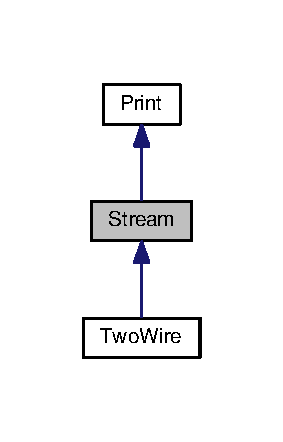
\includegraphics[width=136pt]{class_stream__inherit__graph}
\end{center}
\end{figure}


Collaboration diagram for Stream\+:\nopagebreak
\begin{figure}[H]
\begin{center}
\leavevmode
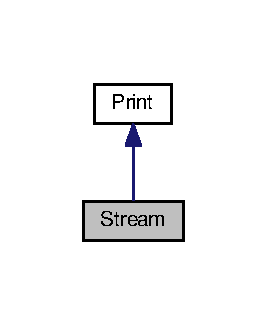
\includegraphics[width=128pt]{class_stream__coll__graph}
\end{center}
\end{figure}
\subsection*{Classes}
\begin{DoxyCompactItemize}
\item 
struct \hyperlink{struct_stream_1_1_multi_target}{Multi\+Target}
\end{DoxyCompactItemize}
\subsection*{Public Member Functions}
\begin{DoxyCompactItemize}
\item 
virtual int {\bfseries available} ()=0\hypertarget{class_stream_a9c98a763395005c08ce95afb2f06c7b1}{}\label{class_stream_a9c98a763395005c08ce95afb2f06c7b1}

\item 
virtual int {\bfseries read} ()=0\hypertarget{class_stream_aea5dee9fcb038148515b7c9212d38dc0}{}\label{class_stream_aea5dee9fcb038148515b7c9212d38dc0}

\item 
virtual int {\bfseries peek} ()=0\hypertarget{class_stream_a30c3c212ec6ea67277a708c5ea2501a5}{}\label{class_stream_a30c3c212ec6ea67277a708c5ea2501a5}

\item 
virtual void {\bfseries flush} ()=0\hypertarget{class_stream_aa3ef2c34f152a0b2ea8de9139b9461da}{}\label{class_stream_aa3ef2c34f152a0b2ea8de9139b9461da}

\item 
void {\bfseries set\+Timeout} (unsigned long timeout)\hypertarget{class_stream_a851dd6dc74d52389de04f99648478db5}{}\label{class_stream_a851dd6dc74d52389de04f99648478db5}

\item 
unsigned long {\bfseries get\+Timeout} (void)\hypertarget{class_stream_abc982d9972a4c7fdabcf7ba9ab325ed1}{}\label{class_stream_abc982d9972a4c7fdabcf7ba9ab325ed1}

\item 
bool {\bfseries find} (char $\ast$target)\hypertarget{class_stream_a4bab30ccd324efd461dee46a2339f673}{}\label{class_stream_a4bab30ccd324efd461dee46a2339f673}

\item 
bool {\bfseries find} (uint8\+\_\+t $\ast$target)\hypertarget{class_stream_a250f5e805979bad3efb0ef33038de457}{}\label{class_stream_a250f5e805979bad3efb0ef33038de457}

\item 
bool {\bfseries find} (char $\ast$target, size\+\_\+t length)\hypertarget{class_stream_ad851401f2318cdb1de05707e021b81d9}{}\label{class_stream_ad851401f2318cdb1de05707e021b81d9}

\item 
bool {\bfseries find} (uint8\+\_\+t $\ast$target, size\+\_\+t length)\hypertarget{class_stream_abe254745b98af8037d10fef6126e42df}{}\label{class_stream_abe254745b98af8037d10fef6126e42df}

\item 
bool {\bfseries find} (char target)\hypertarget{class_stream_a4f529a9d7309aedf535fb1a6757a5675}{}\label{class_stream_a4f529a9d7309aedf535fb1a6757a5675}

\item 
bool {\bfseries find\+Until} (char $\ast$target, char $\ast$terminator)\hypertarget{class_stream_ad1f5f6600832396fb38a897baf4de35b}{}\label{class_stream_ad1f5f6600832396fb38a897baf4de35b}

\item 
bool {\bfseries find\+Until} (uint8\+\_\+t $\ast$target, char $\ast$terminator)\hypertarget{class_stream_a167c5236fd76df40d4894aa48e99aa98}{}\label{class_stream_a167c5236fd76df40d4894aa48e99aa98}

\item 
bool {\bfseries find\+Until} (char $\ast$target, size\+\_\+t target\+Len, char $\ast$terminate, size\+\_\+t term\+Len)\hypertarget{class_stream_a3a9497de614792103ab8cb4759e01a69}{}\label{class_stream_a3a9497de614792103ab8cb4759e01a69}

\item 
bool {\bfseries find\+Until} (uint8\+\_\+t $\ast$target, size\+\_\+t target\+Len, char $\ast$terminate, size\+\_\+t term\+Len)\hypertarget{class_stream_ae644144154e17da36a1b89123847b5b1}{}\label{class_stream_ae644144154e17da36a1b89123847b5b1}

\item 
long {\bfseries parse\+Int} (Lookahead\+Mode lookahead=S\+K\+I\+P\+\_\+\+A\+LL, char ignore=N\+O\+\_\+\+I\+G\+N\+O\+R\+E\+\_\+\+C\+H\+AR)\hypertarget{class_stream_a8875d87ed4db36c36990b2fb22ca48da}{}\label{class_stream_a8875d87ed4db36c36990b2fb22ca48da}

\item 
float {\bfseries parse\+Float} (Lookahead\+Mode lookahead=S\+K\+I\+P\+\_\+\+A\+LL, char ignore=N\+O\+\_\+\+I\+G\+N\+O\+R\+E\+\_\+\+C\+H\+AR)\hypertarget{class_stream_a685133574afc1c35223e31703543a0a7}{}\label{class_stream_a685133574afc1c35223e31703543a0a7}

\item 
size\+\_\+t {\bfseries read\+Bytes} (char $\ast$buffer, size\+\_\+t length)\hypertarget{class_stream_a45fd1336a323ea83b16e8507055f44ea}{}\label{class_stream_a45fd1336a323ea83b16e8507055f44ea}

\item 
size\+\_\+t {\bfseries read\+Bytes} (uint8\+\_\+t $\ast$buffer, size\+\_\+t length)\hypertarget{class_stream_a23dd7428e78e86ff41fce45bd618e214}{}\label{class_stream_a23dd7428e78e86ff41fce45bd618e214}

\item 
size\+\_\+t {\bfseries read\+Bytes\+Until} (char terminator, char $\ast$buffer, size\+\_\+t length)\hypertarget{class_stream_af84672a4fb2620466958d3118d4fea00}{}\label{class_stream_af84672a4fb2620466958d3118d4fea00}

\item 
size\+\_\+t {\bfseries read\+Bytes\+Until} (char terminator, uint8\+\_\+t $\ast$buffer, size\+\_\+t length)\hypertarget{class_stream_a432e1b8520b03a845264789fcb9c1a10}{}\label{class_stream_a432e1b8520b03a845264789fcb9c1a10}

\item 
String {\bfseries read\+String} ()\hypertarget{class_stream_a1c60bdda2b65d78e5a1362d51b856c5a}{}\label{class_stream_a1c60bdda2b65d78e5a1362d51b856c5a}

\item 
String {\bfseries read\+String\+Until} (char terminator)\hypertarget{class_stream_a6a409da87c552909260d8cc428c5ca70}{}\label{class_stream_a6a409da87c552909260d8cc428c5ca70}

\end{DoxyCompactItemize}
\subsection*{Protected Member Functions}
\begin{DoxyCompactItemize}
\item 
int {\bfseries timed\+Read} ()\hypertarget{class_stream_a416a0ada5ed3c9d27f1e72c7d73f0aa1}{}\label{class_stream_a416a0ada5ed3c9d27f1e72c7d73f0aa1}

\item 
int {\bfseries timed\+Peek} ()\hypertarget{class_stream_ae326bf60a3c5276836526710871046fe}{}\label{class_stream_ae326bf60a3c5276836526710871046fe}

\item 
int {\bfseries peek\+Next\+Digit} (Lookahead\+Mode lookahead, bool detect\+Decimal)\hypertarget{class_stream_a3dbc4937689c81b76f4ab16e253e85e0}{}\label{class_stream_a3dbc4937689c81b76f4ab16e253e85e0}

\item 
long {\bfseries parse\+Int} (char ignore)\hypertarget{class_stream_ae37760d5dbfe38e9b9ab403d304c51d8}{}\label{class_stream_ae37760d5dbfe38e9b9ab403d304c51d8}

\item 
float {\bfseries parse\+Float} (char ignore)\hypertarget{class_stream_a5dcf499b28028a5c76f5f9cfe1b73785}{}\label{class_stream_a5dcf499b28028a5c76f5f9cfe1b73785}

\item 
int {\bfseries find\+Multi} (struct \hyperlink{struct_stream_1_1_multi_target}{Multi\+Target} $\ast$targets, int t\+Count)\hypertarget{class_stream_a5fb669d95dbf5b7b8a8e900c53d62a1e}{}\label{class_stream_a5fb669d95dbf5b7b8a8e900c53d62a1e}

\end{DoxyCompactItemize}
\subsection*{Protected Attributes}
\begin{DoxyCompactItemize}
\item 
unsigned long {\bfseries \+\_\+timeout}\hypertarget{class_stream_aae48f1a926d2e82a452f2c75af0c6a29}{}\label{class_stream_aae48f1a926d2e82a452f2c75af0c6a29}

\item 
unsigned long {\bfseries \+\_\+start\+Millis}\hypertarget{class_stream_abf61d2006d28d18f2e028285a323fe5a}{}\label{class_stream_abf61d2006d28d18f2e028285a323fe5a}

\end{DoxyCompactItemize}


The documentation for this class was generated from the following files\+:\begin{DoxyCompactItemize}
\item 
/home/alex/workspace/goldboard4/libs/goldboard4/Stream.\+h\item 
/home/alex/workspace/goldboard4/libs/goldboard4/Stream.\+cpp\end{DoxyCompactItemize}

\hypertarget{class_t_pixy}{}\section{T\+Pixy$<$ Link\+Type $>$ Class Template Reference}
\label{class_t_pixy}\index{T\+Pixy$<$ Link\+Type $>$@{T\+Pixy$<$ Link\+Type $>$}}


Collaboration diagram for T\+Pixy$<$ Link\+Type $>$\+:
\nopagebreak
\begin{figure}[H]
\begin{center}
\leavevmode
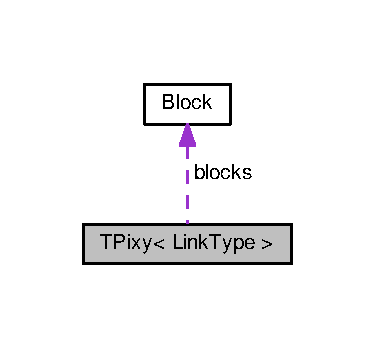
\includegraphics[width=180pt]{class_t_pixy__coll__graph}
\end{center}
\end{figure}
\subsection*{Public Member Functions}
\begin{DoxyCompactItemize}
\item 
{\bfseries T\+Pixy} (uint16\+\_\+t arg=P\+I\+X\+Y\+\_\+\+D\+E\+F\+A\+U\+L\+T\+\_\+\+A\+R\+G\+V\+AL)\hypertarget{class_t_pixy_a6d28834f2de08fc0dd514e854d91c963}{}\label{class_t_pixy_a6d28834f2de08fc0dd514e854d91c963}

\item 
uint16\+\_\+t {\bfseries get\+Blocks} (uint16\+\_\+t max\+Blocks=1000)\hypertarget{class_t_pixy_adea9ba4b37f132747ced41d1a398171b}{}\label{class_t_pixy_adea9ba4b37f132747ced41d1a398171b}

\item 
int8\+\_\+t {\bfseries set\+Servos} (uint16\+\_\+t s0, uint16\+\_\+t s1)\hypertarget{class_t_pixy_a8d768d7d679742d487a44a6af85ccecd}{}\label{class_t_pixy_a8d768d7d679742d487a44a6af85ccecd}

\item 
int8\+\_\+t {\bfseries set\+Brightness} (uint8\+\_\+t brightness)\hypertarget{class_t_pixy_a8c9f442eff27c2fd563da0df9d397d42}{}\label{class_t_pixy_a8c9f442eff27c2fd563da0df9d397d42}

\item 
int8\+\_\+t {\bfseries set\+L\+ED} (uint8\+\_\+t r, uint8\+\_\+t g, uint8\+\_\+t b)\hypertarget{class_t_pixy_a938f7b3d42778ecf8bff8f6eb58ff1c8}{}\label{class_t_pixy_a938f7b3d42778ecf8bff8f6eb58ff1c8}

\item 
void {\bfseries init} ()\hypertarget{class_t_pixy_a9cfbacc18dd014a52926a0239927e29a}{}\label{class_t_pixy_a9cfbacc18dd014a52926a0239927e29a}

\end{DoxyCompactItemize}
\subsection*{Public Attributes}
\begin{DoxyCompactItemize}
\item 
\hyperlink{struct_block}{Block} $\ast$ {\bfseries blocks}\hypertarget{class_t_pixy_a3b56576a5135c7209b834b40869eff6a}{}\label{class_t_pixy_a3b56576a5135c7209b834b40869eff6a}

\end{DoxyCompactItemize}


The documentation for this class was generated from the following file\+:\begin{DoxyCompactItemize}
\item 
/home/alex/workspace/goldboard4/goldboard/T\+Pixy.\+h\end{DoxyCompactItemize}

\hypertarget{class_two_wire}{}\section{Two\+Wire Class Reference}
\label{class_two_wire}\index{Two\+Wire@{Two\+Wire}}


Inheritance diagram for Two\+Wire\+:
\nopagebreak
\begin{figure}[H]
\begin{center}
\leavevmode
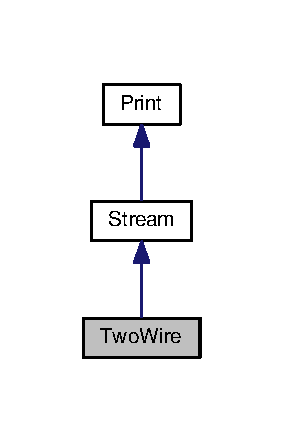
\includegraphics[width=136pt]{class_two_wire__inherit__graph}
\end{center}
\end{figure}


Collaboration diagram for Two\+Wire\+:
\nopagebreak
\begin{figure}[H]
\begin{center}
\leavevmode
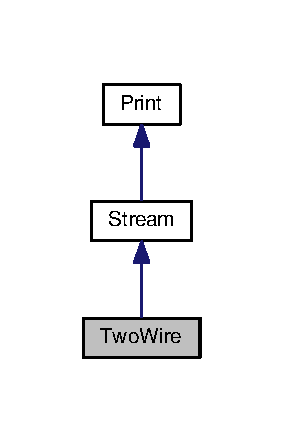
\includegraphics[width=136pt]{class_two_wire__coll__graph}
\end{center}
\end{figure}
\subsection*{Public Member Functions}
\begin{DoxyCompactItemize}
\item 
void {\bfseries begin} ()\hypertarget{class_two_wire_ada85a7a8663ec8af0a1248b659be2f18}{}\label{class_two_wire_ada85a7a8663ec8af0a1248b659be2f18}

\item 
void {\bfseries begin} (uint8\+\_\+t)\hypertarget{class_two_wire_a28bca087ed188781ef15e72622d3b1fb}{}\label{class_two_wire_a28bca087ed188781ef15e72622d3b1fb}

\item 
void {\bfseries begin} (int)\hypertarget{class_two_wire_a2806aa5684d36d7d20bf7c51cab3e602}{}\label{class_two_wire_a2806aa5684d36d7d20bf7c51cab3e602}

\item 
void {\bfseries end} ()\hypertarget{class_two_wire_a13cca813f6dd0201ac70178b18ba0946}{}\label{class_two_wire_a13cca813f6dd0201ac70178b18ba0946}

\item 
void {\bfseries set\+Clock} (uint32\+\_\+t)\hypertarget{class_two_wire_a3c4aaae8779a8c34d8a1a90ff317d982}{}\label{class_two_wire_a3c4aaae8779a8c34d8a1a90ff317d982}

\item 
void {\bfseries begin\+Transmission} (uint8\+\_\+t)\hypertarget{class_two_wire_a8d55f00ea8ac3d7427d62e0c71e95ec2}{}\label{class_two_wire_a8d55f00ea8ac3d7427d62e0c71e95ec2}

\item 
void {\bfseries begin\+Transmission} (int)\hypertarget{class_two_wire_a4da95eb4adced5dad152344243e57aad}{}\label{class_two_wire_a4da95eb4adced5dad152344243e57aad}

\item 
uint8\+\_\+t {\bfseries end\+Transmission} (void)\hypertarget{class_two_wire_af80f9a7b85a3a81a035ca94c95bcdc1d}{}\label{class_two_wire_af80f9a7b85a3a81a035ca94c95bcdc1d}

\item 
uint8\+\_\+t {\bfseries end\+Transmission} (uint8\+\_\+t)\hypertarget{class_two_wire_a289f5ef9bb0f79b31095fd72402ed54a}{}\label{class_two_wire_a289f5ef9bb0f79b31095fd72402ed54a}

\item 
uint8\+\_\+t {\bfseries request\+From} (uint8\+\_\+t, uint8\+\_\+t)\hypertarget{class_two_wire_ae27d0936487551a05a1e9901bc456599}{}\label{class_two_wire_ae27d0936487551a05a1e9901bc456599}

\item 
uint8\+\_\+t {\bfseries request\+From} (uint8\+\_\+t, uint8\+\_\+t, uint8\+\_\+t)\hypertarget{class_two_wire_a4b4b618531a04d5488a52583a3dfb173}{}\label{class_two_wire_a4b4b618531a04d5488a52583a3dfb173}

\item 
uint8\+\_\+t {\bfseries request\+From} (uint8\+\_\+t, uint8\+\_\+t, uint32\+\_\+t, uint8\+\_\+t, uint8\+\_\+t)\hypertarget{class_two_wire_acd59cc9570fd49b1cf9044cbefef85ac}{}\label{class_two_wire_acd59cc9570fd49b1cf9044cbefef85ac}

\item 
uint8\+\_\+t {\bfseries request\+From} (int, int)\hypertarget{class_two_wire_ad40a27213d0bb32f7b819aa8962fccd3}{}\label{class_two_wire_ad40a27213d0bb32f7b819aa8962fccd3}

\item 
uint8\+\_\+t {\bfseries request\+From} (int, int, int)\hypertarget{class_two_wire_a3d76da36fb8571e0b5e8310e9f86f6fe}{}\label{class_two_wire_a3d76da36fb8571e0b5e8310e9f86f6fe}

\item 
virtual size\+\_\+t {\bfseries write} (uint8\+\_\+t)\hypertarget{class_two_wire_a318b7bec156c1f1075a818c0ad3427d7}{}\label{class_two_wire_a318b7bec156c1f1075a818c0ad3427d7}

\item 
virtual size\+\_\+t {\bfseries write} (const uint8\+\_\+t $\ast$, size\+\_\+t)\hypertarget{class_two_wire_a1957b4d5a6a997bdde436e9e40d131a7}{}\label{class_two_wire_a1957b4d5a6a997bdde436e9e40d131a7}

\item 
virtual int {\bfseries available} (void)\hypertarget{class_two_wire_aee57bc52bee06508e231c5fc6bc35ada}{}\label{class_two_wire_aee57bc52bee06508e231c5fc6bc35ada}

\item 
virtual int {\bfseries read} (void)\hypertarget{class_two_wire_aa361b83500d00dfb93bb25b6473b33e9}{}\label{class_two_wire_aa361b83500d00dfb93bb25b6473b33e9}

\item 
virtual int {\bfseries peek} (void)\hypertarget{class_two_wire_a5bd64cb7bd609e9470a15d96a0991ec8}{}\label{class_two_wire_a5bd64cb7bd609e9470a15d96a0991ec8}

\item 
virtual void {\bfseries flush} (void)\hypertarget{class_two_wire_a4d92ddf6ca349c815de1de15fca06b5e}{}\label{class_two_wire_a4d92ddf6ca349c815de1de15fca06b5e}

\item 
void {\bfseries on\+Receive} (void($\ast$)(int))\hypertarget{class_two_wire_a860d97eb825c6fdca388f2f0577cc34a}{}\label{class_two_wire_a860d97eb825c6fdca388f2f0577cc34a}

\item 
void {\bfseries on\+Request} (void($\ast$)(void))\hypertarget{class_two_wire_a224bf8799dda398fc0db223801852ca5}{}\label{class_two_wire_a224bf8799dda398fc0db223801852ca5}

\item 
size\+\_\+t {\bfseries write} (unsigned long n)\hypertarget{class_two_wire_a0c9d09ead8fcddf2a84781fe77d3c975}{}\label{class_two_wire_a0c9d09ead8fcddf2a84781fe77d3c975}

\item 
size\+\_\+t {\bfseries write} (long n)\hypertarget{class_two_wire_a55a9894186458e43852f6fb7c59bb066}{}\label{class_two_wire_a55a9894186458e43852f6fb7c59bb066}

\item 
size\+\_\+t {\bfseries write} (unsigned int n)\hypertarget{class_two_wire_afdb917746ee37f72e7452b4782e9527b}{}\label{class_two_wire_afdb917746ee37f72e7452b4782e9527b}

\item 
size\+\_\+t {\bfseries write} (int n)\hypertarget{class_two_wire_a8ec34b0d2a75e8b2751eb9f4332bd7c3}{}\label{class_two_wire_a8ec34b0d2a75e8b2751eb9f4332bd7c3}

\end{DoxyCompactItemize}
\subsection*{Additional Inherited Members}


The documentation for this class was generated from the following files\+:\begin{DoxyCompactItemize}
\item 
/home/alex/workspace/goldboard4/goldboard/Wire.\+h\item 
/home/alex/workspace/goldboard4/goldboard/Wire.\+cpp\end{DoxyCompactItemize}

\hypertarget{classusring}{}\section{usring Class Reference}
\label{classusring}\index{usring@{usring}}
\subsection*{Public Member Functions}
\begin{DoxyCompactItemize}
\item 
void {\bfseries init} ()\hypertarget{classusring_a321d443eba1e0d0a8d934ed2bd2b62ef}{}\label{classusring_a321d443eba1e0d0a8d934ed2bd2b62ef}

\item 
bool {\bfseries is\+Initialized} ()\hypertarget{classusring_a88b48bd55933924d38f2c2ea0956d529}{}\label{classusring_a88b48bd55933924d38f2c2ea0956d529}

\item 
uint16\+\_\+t {\bfseries get\+Value} ()\hypertarget{classusring_aef8cbedfd02e29767ed71a8da45938a1}{}\label{classusring_aef8cbedfd02e29767ed71a8da45938a1}

\item 
uint8\+\_\+t {\bfseries getanalog\+Value} (uint8\+\_\+t id)\hypertarget{classusring_a79e46727af047f6d2181173f68daae3c}{}\label{classusring_a79e46727af047f6d2181173f68daae3c}

\item 
uint8\+\_\+t {\bfseries get\+Threshold\+Value} (uint8\+\_\+t id)\hypertarget{classusring_a230d462e28252d2029cc70e40d6289fd}{}\label{classusring_a230d462e28252d2029cc70e40d6289fd}

\item 
void {\bfseries set\+Threshold\+Value} (uint8\+\_\+t id, uint8\+\_\+t th)\hypertarget{classusring_a0498d60f7e7908b132968deca273dbf0}{}\label{classusring_a0498d60f7e7908b132968deca273dbf0}

\item 
void {\bfseries set\+Threshold\+Value\+Golbal} (uint8\+\_\+t th)\hypertarget{classusring_a67e0e2972434462c28b9abfbe44da941}{}\label{classusring_a67e0e2972434462c28b9abfbe44da941}

\item 
bool {\bfseries check\+Ack} ()\hypertarget{classusring_abc14d72023af94ffdba22b101a5d9152}{}\label{classusring_abc14d72023af94ffdba22b101a5d9152}

\end{DoxyCompactItemize}


The documentation for this class was generated from the following files\+:\begin{DoxyCompactItemize}
\item 
/home/alex/workspace/goldboard4/libs/goldboard4/usring.\+h\item 
/home/alex/workspace/goldboard4/libs/goldboard4/usring.\+cpp\end{DoxyCompactItemize}

\hypertarget{class_v_l53_l0_x}{}\section{V\+L53\+L0X Class Reference}
\label{class_v_l53_l0_x}\index{V\+L53\+L0X@{V\+L53\+L0X}}
\subsection*{Public Types}
\begin{DoxyCompactItemize}
\item 
enum {\bfseries reg\+Addr} \{ \\*
{\bfseries S\+Y\+S\+R\+A\+N\+G\+E\+\_\+\+S\+T\+A\+RT} = 0x00, 
{\bfseries S\+Y\+S\+T\+E\+M\+\_\+\+T\+H\+R\+E\+S\+H\+\_\+\+H\+I\+GH} = 0x0C, 
{\bfseries S\+Y\+S\+T\+E\+M\+\_\+\+T\+H\+R\+E\+S\+H\+\_\+\+L\+OW} = 0x0E, 
{\bfseries S\+Y\+S\+T\+E\+M\+\_\+\+S\+E\+Q\+U\+E\+N\+C\+E\+\_\+\+C\+O\+N\+F\+IG} = 0x01, 
\\*
{\bfseries S\+Y\+S\+T\+E\+M\+\_\+\+R\+A\+N\+G\+E\+\_\+\+C\+O\+N\+F\+IG} = 0x09, 
{\bfseries S\+Y\+S\+T\+E\+M\+\_\+\+I\+N\+T\+E\+R\+M\+E\+A\+S\+U\+R\+E\+M\+E\+N\+T\+\_\+\+P\+E\+R\+I\+OD} = 0x04, 
{\bfseries S\+Y\+S\+T\+E\+M\+\_\+\+I\+N\+T\+E\+R\+R\+U\+P\+T\+\_\+\+C\+O\+N\+F\+I\+G\+\_\+\+G\+P\+IO} = 0x0A, 
{\bfseries G\+P\+I\+O\+\_\+\+H\+V\+\_\+\+M\+U\+X\+\_\+\+A\+C\+T\+I\+V\+E\+\_\+\+H\+I\+GH} = 0x84, 
\\*
{\bfseries S\+Y\+S\+T\+E\+M\+\_\+\+I\+N\+T\+E\+R\+R\+U\+P\+T\+\_\+\+C\+L\+E\+AR} = 0x0B, 
{\bfseries R\+E\+S\+U\+L\+T\+\_\+\+I\+N\+T\+E\+R\+R\+U\+P\+T\+\_\+\+S\+T\+A\+T\+US} = 0x13, 
{\bfseries R\+E\+S\+U\+L\+T\+\_\+\+R\+A\+N\+G\+E\+\_\+\+S\+T\+A\+T\+US} = 0x14, 
{\bfseries R\+E\+S\+U\+L\+T\+\_\+\+C\+O\+R\+E\+\_\+\+A\+M\+B\+I\+E\+N\+T\+\_\+\+W\+I\+N\+D\+O\+W\+\_\+\+E\+V\+E\+N\+T\+S\+\_\+\+R\+TN} = 0x\+BC, 
\\*
{\bfseries R\+E\+S\+U\+L\+T\+\_\+\+C\+O\+R\+E\+\_\+\+R\+A\+N\+G\+I\+N\+G\+\_\+\+T\+O\+T\+A\+L\+\_\+\+E\+V\+E\+N\+T\+S\+\_\+\+R\+TN} = 0x\+C0, 
{\bfseries R\+E\+S\+U\+L\+T\+\_\+\+C\+O\+R\+E\+\_\+\+A\+M\+B\+I\+E\+N\+T\+\_\+\+W\+I\+N\+D\+O\+W\+\_\+\+E\+V\+E\+N\+T\+S\+\_\+\+R\+EF} = 0x\+D0, 
{\bfseries R\+E\+S\+U\+L\+T\+\_\+\+C\+O\+R\+E\+\_\+\+R\+A\+N\+G\+I\+N\+G\+\_\+\+T\+O\+T\+A\+L\+\_\+\+E\+V\+E\+N\+T\+S\+\_\+\+R\+EF} = 0x\+D4, 
{\bfseries R\+E\+S\+U\+L\+T\+\_\+\+P\+E\+A\+K\+\_\+\+S\+I\+G\+N\+A\+L\+\_\+\+R\+A\+T\+E\+\_\+\+R\+EF} = 0x\+B6, 
\\*
{\bfseries A\+L\+G\+O\+\_\+\+P\+A\+R\+T\+\_\+\+T\+O\+\_\+\+P\+A\+R\+T\+\_\+\+R\+A\+N\+G\+E\+\_\+\+O\+F\+F\+S\+E\+T\+\_\+\+MM} = 0x28, 
{\bfseries I2\+C\+\_\+\+S\+L\+A\+V\+E\+\_\+\+D\+E\+V\+I\+C\+E\+\_\+\+A\+D\+D\+R\+E\+SS} = 0x8A, 
{\bfseries M\+S\+R\+C\+\_\+\+C\+O\+N\+F\+I\+G\+\_\+\+C\+O\+N\+T\+R\+OL} = 0x60, 
{\bfseries P\+R\+E\+\_\+\+R\+A\+N\+G\+E\+\_\+\+C\+O\+N\+F\+I\+G\+\_\+\+M\+I\+N\+\_\+\+S\+NR} = 0x27, 
\\*
{\bfseries P\+R\+E\+\_\+\+R\+A\+N\+G\+E\+\_\+\+C\+O\+N\+F\+I\+G\+\_\+\+V\+A\+L\+I\+D\+\_\+\+P\+H\+A\+S\+E\+\_\+\+L\+OW} = 0x56, 
{\bfseries P\+R\+E\+\_\+\+R\+A\+N\+G\+E\+\_\+\+C\+O\+N\+F\+I\+G\+\_\+\+V\+A\+L\+I\+D\+\_\+\+P\+H\+A\+S\+E\+\_\+\+H\+I\+GH} = 0x57, 
{\bfseries P\+R\+E\+\_\+\+R\+A\+N\+G\+E\+\_\+\+M\+I\+N\+\_\+\+C\+O\+U\+N\+T\+\_\+\+R\+A\+T\+E\+\_\+\+R\+T\+N\+\_\+\+L\+I\+M\+IT} = 0x64, 
{\bfseries F\+I\+N\+A\+L\+\_\+\+R\+A\+N\+G\+E\+\_\+\+C\+O\+N\+F\+I\+G\+\_\+\+M\+I\+N\+\_\+\+S\+NR} = 0x67, 
\\*
{\bfseries F\+I\+N\+A\+L\+\_\+\+R\+A\+N\+G\+E\+\_\+\+C\+O\+N\+F\+I\+G\+\_\+\+V\+A\+L\+I\+D\+\_\+\+P\+H\+A\+S\+E\+\_\+\+L\+OW} = 0x47, 
{\bfseries F\+I\+N\+A\+L\+\_\+\+R\+A\+N\+G\+E\+\_\+\+C\+O\+N\+F\+I\+G\+\_\+\+V\+A\+L\+I\+D\+\_\+\+P\+H\+A\+S\+E\+\_\+\+H\+I\+GH} = 0x48, 
{\bfseries F\+I\+N\+A\+L\+\_\+\+R\+A\+N\+G\+E\+\_\+\+C\+O\+N\+F\+I\+G\+\_\+\+M\+I\+N\+\_\+\+C\+O\+U\+N\+T\+\_\+\+R\+A\+T\+E\+\_\+\+R\+T\+N\+\_\+\+L\+I\+M\+IT} = 0x44, 
{\bfseries P\+R\+E\+\_\+\+R\+A\+N\+G\+E\+\_\+\+C\+O\+N\+F\+I\+G\+\_\+\+S\+I\+G\+M\+A\+\_\+\+T\+H\+R\+E\+S\+H\+\_\+\+HI} = 0x61, 
\\*
{\bfseries P\+R\+E\+\_\+\+R\+A\+N\+G\+E\+\_\+\+C\+O\+N\+F\+I\+G\+\_\+\+S\+I\+G\+M\+A\+\_\+\+T\+H\+R\+E\+S\+H\+\_\+\+LO} = 0x62, 
{\bfseries P\+R\+E\+\_\+\+R\+A\+N\+G\+E\+\_\+\+C\+O\+N\+F\+I\+G\+\_\+\+V\+C\+S\+E\+L\+\_\+\+P\+E\+R\+I\+OD} = 0x50, 
{\bfseries P\+R\+E\+\_\+\+R\+A\+N\+G\+E\+\_\+\+C\+O\+N\+F\+I\+G\+\_\+\+T\+I\+M\+E\+O\+U\+T\+\_\+\+M\+A\+C\+R\+O\+P\+\_\+\+HI} = 0x51, 
{\bfseries P\+R\+E\+\_\+\+R\+A\+N\+G\+E\+\_\+\+C\+O\+N\+F\+I\+G\+\_\+\+T\+I\+M\+E\+O\+U\+T\+\_\+\+M\+A\+C\+R\+O\+P\+\_\+\+LO} = 0x52, 
\\*
{\bfseries S\+Y\+S\+T\+E\+M\+\_\+\+H\+I\+S\+T\+O\+G\+R\+A\+M\+\_\+\+B\+IN} = 0x81, 
{\bfseries H\+I\+S\+T\+O\+G\+R\+A\+M\+\_\+\+C\+O\+N\+F\+I\+G\+\_\+\+I\+N\+I\+T\+I\+A\+L\+\_\+\+P\+H\+A\+S\+E\+\_\+\+S\+E\+L\+E\+CT} = 0x33, 
{\bfseries H\+I\+S\+T\+O\+G\+R\+A\+M\+\_\+\+C\+O\+N\+F\+I\+G\+\_\+\+R\+E\+A\+D\+O\+U\+T\+\_\+\+C\+T\+RL} = 0x55, 
{\bfseries F\+I\+N\+A\+L\+\_\+\+R\+A\+N\+G\+E\+\_\+\+C\+O\+N\+F\+I\+G\+\_\+\+V\+C\+S\+E\+L\+\_\+\+P\+E\+R\+I\+OD} = 0x70, 
\\*
{\bfseries F\+I\+N\+A\+L\+\_\+\+R\+A\+N\+G\+E\+\_\+\+C\+O\+N\+F\+I\+G\+\_\+\+T\+I\+M\+E\+O\+U\+T\+\_\+\+M\+A\+C\+R\+O\+P\+\_\+\+HI} = 0x71, 
{\bfseries F\+I\+N\+A\+L\+\_\+\+R\+A\+N\+G\+E\+\_\+\+C\+O\+N\+F\+I\+G\+\_\+\+T\+I\+M\+E\+O\+U\+T\+\_\+\+M\+A\+C\+R\+O\+P\+\_\+\+LO} = 0x72, 
{\bfseries C\+R\+O\+S\+S\+T\+A\+L\+K\+\_\+\+C\+O\+M\+P\+E\+N\+S\+A\+T\+I\+O\+N\+\_\+\+P\+E\+A\+K\+\_\+\+R\+A\+T\+E\+\_\+\+M\+C\+PS} = 0x20, 
{\bfseries M\+S\+R\+C\+\_\+\+C\+O\+N\+F\+I\+G\+\_\+\+T\+I\+M\+E\+O\+U\+T\+\_\+\+M\+A\+C\+R\+OP} = 0x46, 
\\*
{\bfseries S\+O\+F\+T\+\_\+\+R\+E\+S\+E\+T\+\_\+\+G\+O2\+\_\+\+S\+O\+F\+T\+\_\+\+R\+E\+S\+E\+T\+\_\+N} = 0x\+BF, 
{\bfseries I\+D\+E\+N\+T\+I\+F\+I\+C\+A\+T\+I\+O\+N\+\_\+\+M\+O\+D\+E\+L\+\_\+\+ID} = 0x\+C0, 
{\bfseries I\+D\+E\+N\+T\+I\+F\+I\+C\+A\+T\+I\+O\+N\+\_\+\+R\+E\+V\+I\+S\+I\+O\+N\+\_\+\+ID} = 0x\+C2, 
{\bfseries O\+S\+C\+\_\+\+C\+A\+L\+I\+B\+R\+A\+T\+E\+\_\+\+V\+AL} = 0x\+F8, 
\\*
{\bfseries G\+L\+O\+B\+A\+L\+\_\+\+C\+O\+N\+F\+I\+G\+\_\+\+V\+C\+S\+E\+L\+\_\+\+W\+I\+D\+TH} = 0x32, 
{\bfseries G\+L\+O\+B\+A\+L\+\_\+\+C\+O\+N\+F\+I\+G\+\_\+\+S\+P\+A\+D\+\_\+\+E\+N\+A\+B\+L\+E\+S\+\_\+\+R\+E\+F\+\_\+0} = 0x\+B0, 
{\bfseries G\+L\+O\+B\+A\+L\+\_\+\+C\+O\+N\+F\+I\+G\+\_\+\+S\+P\+A\+D\+\_\+\+E\+N\+A\+B\+L\+E\+S\+\_\+\+R\+E\+F\+\_\+1} = 0x\+B1, 
{\bfseries G\+L\+O\+B\+A\+L\+\_\+\+C\+O\+N\+F\+I\+G\+\_\+\+S\+P\+A\+D\+\_\+\+E\+N\+A\+B\+L\+E\+S\+\_\+\+R\+E\+F\+\_\+2} = 0x\+B2, 
\\*
{\bfseries G\+L\+O\+B\+A\+L\+\_\+\+C\+O\+N\+F\+I\+G\+\_\+\+S\+P\+A\+D\+\_\+\+E\+N\+A\+B\+L\+E\+S\+\_\+\+R\+E\+F\+\_\+3} = 0x\+B3, 
{\bfseries G\+L\+O\+B\+A\+L\+\_\+\+C\+O\+N\+F\+I\+G\+\_\+\+S\+P\+A\+D\+\_\+\+E\+N\+A\+B\+L\+E\+S\+\_\+\+R\+E\+F\+\_\+4} = 0x\+B4, 
{\bfseries G\+L\+O\+B\+A\+L\+\_\+\+C\+O\+N\+F\+I\+G\+\_\+\+S\+P\+A\+D\+\_\+\+E\+N\+A\+B\+L\+E\+S\+\_\+\+R\+E\+F\+\_\+5} = 0x\+B5, 
{\bfseries G\+L\+O\+B\+A\+L\+\_\+\+C\+O\+N\+F\+I\+G\+\_\+\+R\+E\+F\+\_\+\+E\+N\+\_\+\+S\+T\+A\+R\+T\+\_\+\+S\+E\+L\+E\+CT} = 0x\+B6, 
\\*
{\bfseries D\+Y\+N\+A\+M\+I\+C\+\_\+\+S\+P\+A\+D\+\_\+\+N\+U\+M\+\_\+\+R\+E\+Q\+U\+E\+S\+T\+E\+D\+\_\+\+R\+E\+F\+\_\+\+S\+P\+AD} = 0x4E, 
{\bfseries D\+Y\+N\+A\+M\+I\+C\+\_\+\+S\+P\+A\+D\+\_\+\+R\+E\+F\+\_\+\+E\+N\+\_\+\+S\+T\+A\+R\+T\+\_\+\+O\+F\+F\+S\+ET} = 0x4F, 
{\bfseries P\+O\+W\+E\+R\+\_\+\+M\+A\+N\+A\+G\+E\+M\+E\+N\+T\+\_\+\+G\+O1\+\_\+\+P\+O\+W\+E\+R\+\_\+\+F\+O\+R\+CE} = 0x80, 
{\bfseries V\+H\+V\+\_\+\+C\+O\+N\+F\+I\+G\+\_\+\+P\+A\+D\+\_\+\+S\+C\+L\+\_\+\+S\+D\+A\+\_\+\+\_\+\+E\+X\+T\+S\+U\+P\+\_\+\+HV} = 0x89, 
\\*
{\bfseries A\+L\+G\+O\+\_\+\+P\+H\+A\+S\+E\+C\+A\+L\+\_\+\+L\+IM} = 0x30, 
{\bfseries A\+L\+G\+O\+\_\+\+P\+H\+A\+S\+E\+C\+A\+L\+\_\+\+C\+O\+N\+F\+I\+G\+\_\+\+T\+I\+M\+E\+O\+UT} = 0x30
 \}\hypertarget{class_v_l53_l0_x_ae9d956d60961a009db8621edde00bfea}{}\label{class_v_l53_l0_x_ae9d956d60961a009db8621edde00bfea}

\item 
enum {\bfseries vcsel\+Period\+Type} \{ {\bfseries Vcsel\+Period\+Pre\+Range}, 
{\bfseries Vcsel\+Period\+Final\+Range}
 \}\hypertarget{class_v_l53_l0_x_a536b605b1242dd5355f49273450f8c83}{}\label{class_v_l53_l0_x_a536b605b1242dd5355f49273450f8c83}

\end{DoxyCompactItemize}
\subsection*{Public Member Functions}
\begin{DoxyCompactItemize}
\item 
void {\bfseries set\+Address} (uint8\+\_\+t new\+\_\+addr)\hypertarget{class_v_l53_l0_x_a5fafb26368ff871653f4b56e060606fa}{}\label{class_v_l53_l0_x_a5fafb26368ff871653f4b56e060606fa}

\item 
uint8\+\_\+t {\bfseries get\+Address} (void)\hypertarget{class_v_l53_l0_x_a4bc871502a5635943e3bc5ce06599105}{}\label{class_v_l53_l0_x_a4bc871502a5635943e3bc5ce06599105}

\item 
bool {\bfseries init} (bool io\+\_\+2v8=true)\hypertarget{class_v_l53_l0_x_a2bd7f966631ee954fd1c4119f901b240}{}\label{class_v_l53_l0_x_a2bd7f966631ee954fd1c4119f901b240}

\item 
void {\bfseries write\+Reg} (uint8\+\_\+t reg, uint8\+\_\+t value)\hypertarget{class_v_l53_l0_x_a607bdb2d634b1ec3878dbaee6d83402e}{}\label{class_v_l53_l0_x_a607bdb2d634b1ec3878dbaee6d83402e}

\item 
void {\bfseries write\+Reg16\+Bit} (uint8\+\_\+t reg, uint16\+\_\+t value)\hypertarget{class_v_l53_l0_x_ade0f7181294f755fedd269253a3c4bb4}{}\label{class_v_l53_l0_x_ade0f7181294f755fedd269253a3c4bb4}

\item 
void {\bfseries write\+Reg32\+Bit} (uint8\+\_\+t reg, uint32\+\_\+t value)\hypertarget{class_v_l53_l0_x_aa67924fc9b90b086d667a92bd3195921}{}\label{class_v_l53_l0_x_aa67924fc9b90b086d667a92bd3195921}

\item 
uint8\+\_\+t {\bfseries read\+Reg} (uint8\+\_\+t reg)\hypertarget{class_v_l53_l0_x_a44cad5c80035df82bdc1c28894ac714e}{}\label{class_v_l53_l0_x_a44cad5c80035df82bdc1c28894ac714e}

\item 
uint16\+\_\+t {\bfseries read\+Reg16\+Bit} (uint8\+\_\+t reg)\hypertarget{class_v_l53_l0_x_afa23131ef0c5edc982a3d9ab843fefc8}{}\label{class_v_l53_l0_x_afa23131ef0c5edc982a3d9ab843fefc8}

\item 
uint32\+\_\+t {\bfseries read\+Reg32\+Bit} (uint8\+\_\+t reg)\hypertarget{class_v_l53_l0_x_a8e6edc19a09bff41ac070d22204ce5db}{}\label{class_v_l53_l0_x_a8e6edc19a09bff41ac070d22204ce5db}

\item 
void {\bfseries write\+Multi} (uint8\+\_\+t reg, uint8\+\_\+t const $\ast$src, uint8\+\_\+t count)\hypertarget{class_v_l53_l0_x_a22b4ca7c4e0562ddcb74cc939024deb2}{}\label{class_v_l53_l0_x_a22b4ca7c4e0562ddcb74cc939024deb2}

\item 
void {\bfseries read\+Multi} (uint8\+\_\+t reg, uint8\+\_\+t $\ast$dst, uint8\+\_\+t count)\hypertarget{class_v_l53_l0_x_a9decb4846fd2cc6d9c15b29ff2edc275}{}\label{class_v_l53_l0_x_a9decb4846fd2cc6d9c15b29ff2edc275}

\item 
bool {\bfseries set\+Signal\+Rate\+Limit} (float limit\+\_\+\+Mcps)\hypertarget{class_v_l53_l0_x_a32ea0f8c88d634abcf36850ced40e9eb}{}\label{class_v_l53_l0_x_a32ea0f8c88d634abcf36850ced40e9eb}

\item 
float {\bfseries get\+Signal\+Rate\+Limit} (void)\hypertarget{class_v_l53_l0_x_a5fdac59ab355cc57f27462823cc576d4}{}\label{class_v_l53_l0_x_a5fdac59ab355cc57f27462823cc576d4}

\item 
bool {\bfseries set\+Measurement\+Timing\+Budget} (uint32\+\_\+t budget\+\_\+us)\hypertarget{class_v_l53_l0_x_a74e836308c2062c7871a37fe11c026ca}{}\label{class_v_l53_l0_x_a74e836308c2062c7871a37fe11c026ca}

\item 
uint32\+\_\+t {\bfseries get\+Measurement\+Timing\+Budget} (void)\hypertarget{class_v_l53_l0_x_a9c9cb975a20876bae3d7716c698b72eb}{}\label{class_v_l53_l0_x_a9c9cb975a20876bae3d7716c698b72eb}

\item 
bool {\bfseries set\+Vcsel\+Pulse\+Period} (vcsel\+Period\+Type type, uint8\+\_\+t period\+\_\+pclks)\hypertarget{class_v_l53_l0_x_a2234b48a180b7eb630b7a82cfa4c3b44}{}\label{class_v_l53_l0_x_a2234b48a180b7eb630b7a82cfa4c3b44}

\item 
uint8\+\_\+t {\bfseries get\+Vcsel\+Pulse\+Period} (vcsel\+Period\+Type type)\hypertarget{class_v_l53_l0_x_a1a5b6c572a2be57ae5503ae81fea0f87}{}\label{class_v_l53_l0_x_a1a5b6c572a2be57ae5503ae81fea0f87}

\item 
void {\bfseries start\+Continuous} (uint32\+\_\+t period\+\_\+ms=0)\hypertarget{class_v_l53_l0_x_a502070924e6c6fa39a7a003bdf1c8663}{}\label{class_v_l53_l0_x_a502070924e6c6fa39a7a003bdf1c8663}

\item 
void {\bfseries stop\+Continuous} (void)\hypertarget{class_v_l53_l0_x_aaa035aea7642fbf97e7946a1159ca5a5}{}\label{class_v_l53_l0_x_aaa035aea7642fbf97e7946a1159ca5a5}

\item 
uint16\+\_\+t {\bfseries read\+Range\+Continuous\+Millimeters} (void)\hypertarget{class_v_l53_l0_x_a198b2629c8d805ce23b2b2dd3c3cf7cf}{}\label{class_v_l53_l0_x_a198b2629c8d805ce23b2b2dd3c3cf7cf}

\item 
uint16\+\_\+t {\bfseries read\+Range\+Single\+Millimeters} (void)\hypertarget{class_v_l53_l0_x_a49e5ed380d53cbcedad7b96ec1eadb44}{}\label{class_v_l53_l0_x_a49e5ed380d53cbcedad7b96ec1eadb44}

\item 
void {\bfseries set\+Timeout} (uint16\+\_\+t timeout)\hypertarget{class_v_l53_l0_x_a421ae3c8aaad208e7e8c07c6f88cf486}{}\label{class_v_l53_l0_x_a421ae3c8aaad208e7e8c07c6f88cf486}

\item 
uint16\+\_\+t {\bfseries get\+Timeout} (void)\hypertarget{class_v_l53_l0_x_ac33d634573c44958b28ca42db5df0814}{}\label{class_v_l53_l0_x_ac33d634573c44958b28ca42db5df0814}

\item 
bool {\bfseries timeout\+Occurred} (void)\hypertarget{class_v_l53_l0_x_a7356434e330aa7c4243d75ec5349db5d}{}\label{class_v_l53_l0_x_a7356434e330aa7c4243d75ec5349db5d}

\end{DoxyCompactItemize}
\subsection*{Public Attributes}
\begin{DoxyCompactItemize}
\item 
uint8\+\_\+t {\bfseries last\+\_\+status}\hypertarget{class_v_l53_l0_x_af33d12ec0d1eb8630bb3473c07c2b853}{}\label{class_v_l53_l0_x_af33d12ec0d1eb8630bb3473c07c2b853}

\end{DoxyCompactItemize}


The documentation for this class was generated from the following files\+:\begin{DoxyCompactItemize}
\item 
/home/alex/workspace/goldboard4/libs/goldboard4/V\+L53\+L0\+X.\+h\item 
/home/alex/workspace/goldboard4/libs/goldboard4/V\+L53\+L0\+X.\+cpp\end{DoxyCompactItemize}

\chapter{File Documentation}
\hypertarget{i2c_8h}{}\section{/home/alex/workspace/goldboard4/libs/goldboard4/i2c.h File Reference}
\label{i2c_8h}\index{/home/alex/workspace/goldboard4/libs/goldboard4/i2c.\+h@{/home/alex/workspace/goldboard4/libs/goldboard4/i2c.\+h}}


I2\+C-\/\+Treiber, derzeit nur Master, interruptbasiert.  


{\ttfamily \#include \char`\"{}global.\+h\char`\"{}}\\*
{\ttfamily \#include $<$stdbool.\+h$>$}\\*
{\ttfamily \#include $<$stdlib.\+h$>$}\\*
{\ttfamily \#include $<$util/twi.\+h$>$}\\*
Include dependency graph for i2c.\+h\+:
\nopagebreak
\begin{figure}[H]
\begin{center}
\leavevmode
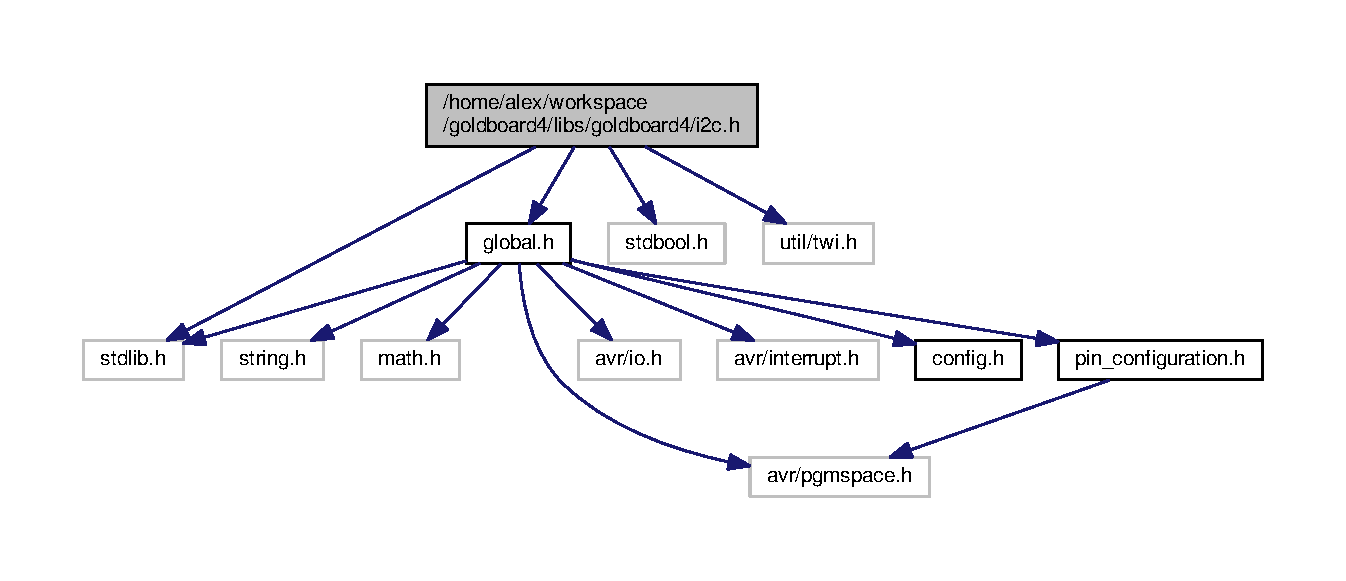
\includegraphics[width=350pt]{i2c_8h__incl}
\end{center}
\end{figure}
This graph shows which files directly or indirectly include this file\+:
\nopagebreak
\begin{figure}[H]
\begin{center}
\leavevmode
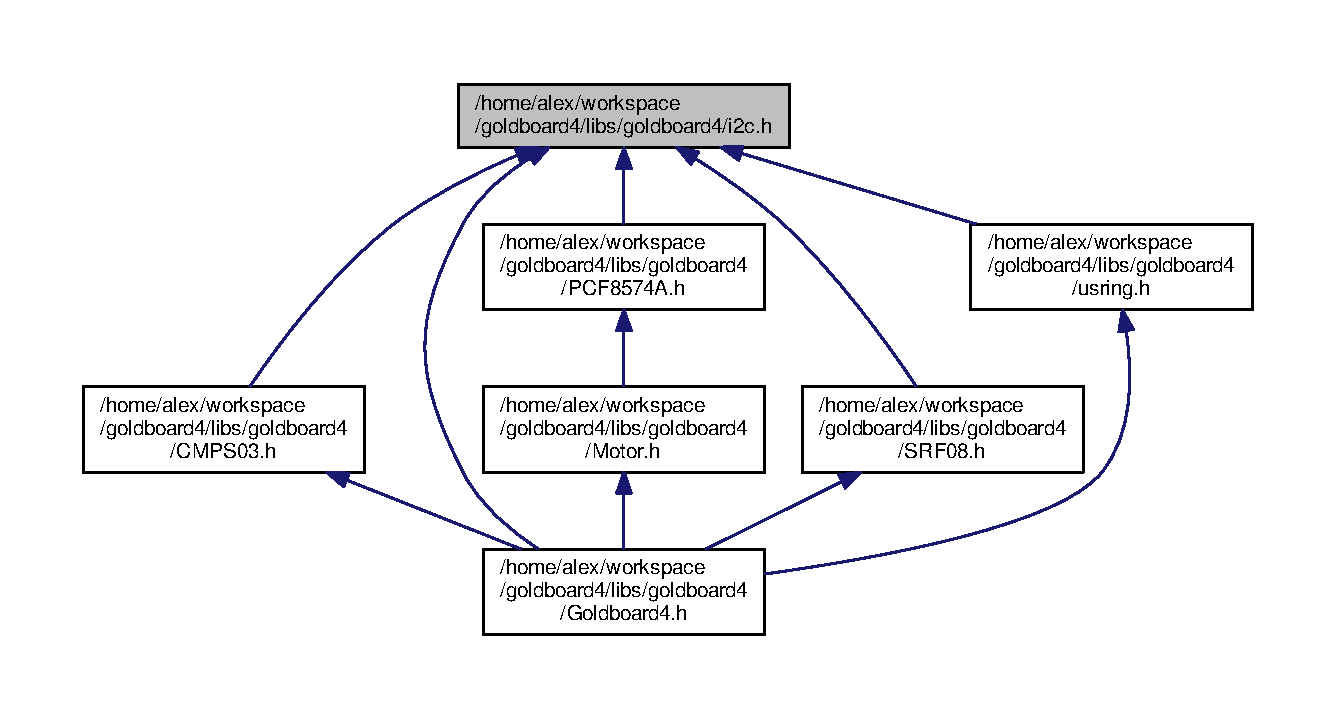
\includegraphics[width=350pt]{i2c_8h__dep__incl}
\end{center}
\end{figure}
\subsection*{Macros}
\begin{DoxyCompactItemize}
\item 
\#define {\bfseries T\+W\+\_\+\+T\+I\+M\+E\+O\+U\+T\+\_\+\+E\+R\+R\+OR}~0x\+FF\hypertarget{i2c_8h_a5cc0a1876a3d4815d6a9a69bce653c04}{}\label{i2c_8h_a5cc0a1876a3d4815d6a9a69bce653c04}

\item 
\#define {\bfseries I2\+C\+\_\+\+O\+N\+\_\+\+E\+R\+R\+O\+R\+\_\+\+F\+A\+T\+AL}\hypertarget{i2c_8h_ad8c710658fa32f2f8974d6d357dcd9c5}{}\label{i2c_8h_ad8c710658fa32f2f8974d6d357dcd9c5}

\end{DoxyCompactItemize}
\subsection*{Functions}
\begin{DoxyCompactItemize}
\item 
boolean \hyperlink{i2c_8h_abc18fd0461e5c6b433285335acac0cc9}{i2c\+Is\+Complete} (void)
\item 
boolean {\bfseries i2c\+Check\+Ack} (uint8\+\_\+t address)\hypertarget{i2c_8h_aaac167b570f1dc5c40e5987a3813af79}{}\label{i2c_8h_aaac167b570f1dc5c40e5987a3813af79}

\item 
uint8\+\_\+t \hyperlink{i2c_8h_a1091488ad34f5e8990091aa6b01fb8c9}{i2c\+Get\+Last\+Error} (void)
\item 
void \hyperlink{i2c_8h_af41a62505fd4ca300eeed25ac1de911c}{i2c\+Init} (uint16\+\_\+t bitrate\+K\+Hz)
\item 
void {\bfseries i2c\+Close} (void)\hypertarget{i2c_8h_a51b2aeb913a9c0512f9ddccf5fa38ea9}{}\label{i2c_8h_a51b2aeb913a9c0512f9ddccf5fa38ea9}

\item 
bool \hyperlink{i2c_8h_ac4d5f5ff28c1f69c741b81e225d16e40}{i2c\+Transfer} (uint8\+\_\+t address, uint8\+\_\+t $\ast$p\+Tx, uint8\+\_\+t n\+Tx, uint8\+\_\+t $\ast$p\+Rx, uint8\+\_\+t n\+Rx)
\item 
bool \hyperlink{i2c_8h_a4c27e5b9ba55b6f1b5acc89d680eccc8}{i2c\+Read} (uint8\+\_\+t address, uint8\+\_\+t reg, uint8\+\_\+t $\ast$p\+Rx, uint8\+\_\+t n\+Rx)
\item 
bool {\bfseries i2c\+Read\+Register} (uint8\+\_\+t address, uint8\+\_\+t reg, uint8\+\_\+t $\ast$data)\hypertarget{i2c_8h_ad5dda112cafeca6dff8f28ce5f74a99c}{}\label{i2c_8h_ad5dda112cafeca6dff8f28ce5f74a99c}

\item 
bool \hyperlink{i2c_8h_a83fbf015492a78db2816a105738d392e}{i2c\+Write\+Register} (uint8\+\_\+t address, uint8\+\_\+t reg, uint8\+\_\+t data)
\item 
bool {\bfseries i2c\+Write\+To\+Slave} (uint8\+\_\+t address, uint8\+\_\+t $\ast$buf, int count)\hypertarget{i2c_8h_a71c6d51fa5ea99f0cd2adffd5cd44508}{}\label{i2c_8h_a71c6d51fa5ea99f0cd2adffd5cd44508}

\item 
uint8\+\_\+t \hyperlink{i2c_8h_a11775628753d9e39e692171f1a88927b}{i2c\+Wait} (void)
\item 
void \hyperlink{i2c_8h_ad7c22c019c4a90ad53ec546a3f8d80a0}{i2c\+Test} (void)
\end{DoxyCompactItemize}


\subsection{Detailed Description}
I2\+C-\/\+Treiber, derzeit nur Master, interruptbasiert. 

\begin{DoxyAuthor}{Author}
Timo Sandmann (\href{mailto:mail@timosandmann.de}{\tt mail@timosandmann.\+de}) 
\end{DoxyAuthor}
\begin{DoxyDate}{Date}
05.\+09.\+2007
\end{DoxyDate}
Changes by Roman Steiger \begin{DoxyDate}{Date}
17.\+01.\+2008 
\end{DoxyDate}


\subsection{Function Documentation}
\index{i2c.\+h@{i2c.\+h}!i2c\+Get\+Last\+Error@{i2c\+Get\+Last\+Error}}
\index{i2c\+Get\+Last\+Error@{i2c\+Get\+Last\+Error}!i2c.\+h@{i2c.\+h}}
\subsubsection[{\texorpdfstring{i2c\+Get\+Last\+Error(void)}{i2cGetLastError(void)}}]{\setlength{\rightskip}{0pt plus 5cm}uint8\+\_\+t i2c\+Get\+Last\+Error (
\begin{DoxyParamCaption}
\item[{void}]{}
\end{DoxyParamCaption}
)\hspace{0.3cm}{\ttfamily [inline]}}\hypertarget{i2c_8h_a1091488ad34f5e8990091aa6b01fb8c9}{}\label{i2c_8h_a1091488ad34f5e8990091aa6b01fb8c9}
T\+W\+\_\+\+N\+O\+\_\+\+I\+N\+FO if no error occured \index{i2c.\+h@{i2c.\+h}!i2c\+Init@{i2c\+Init}}
\index{i2c\+Init@{i2c\+Init}!i2c.\+h@{i2c.\+h}}
\subsubsection[{\texorpdfstring{i2c\+Init(uint16\+\_\+t bitrate\+K\+Hz)}{i2cInit(uint16_t bitrateKHz)}}]{\setlength{\rightskip}{0pt plus 5cm}void i2c\+Init (
\begin{DoxyParamCaption}
\item[{uint16\+\_\+t}]{bitrate\+K\+Hz}
\end{DoxyParamCaption}
)}\hypertarget{i2c_8h_af41a62505fd4ca300eeed25ac1de911c}{}\label{i2c_8h_af41a62505fd4ca300eeed25ac1de911c}
Initialisiert das I2\+C-\/\+Modul 
\begin{DoxyParams}{Parameters}
{\em bitrate} & Init-\/\+Wert in k\+Hz\\
\hline
\end{DoxyParams}
S\+CL frequency = C\+PU Clock frequency / 16 + 2(T\+W\+BR) $\ast$ 4$^\wedge$\+T\+W\+PS � T\+W\+BR = Value of the T\+WI Bit Rate Register � T\+W\+PS = Value of the prescaler bits in the T\+WI Status Register \index{i2c.\+h@{i2c.\+h}!i2c\+Is\+Complete@{i2c\+Is\+Complete}}
\index{i2c\+Is\+Complete@{i2c\+Is\+Complete}!i2c.\+h@{i2c.\+h}}
\subsubsection[{\texorpdfstring{i2c\+Is\+Complete(void)}{i2cIsComplete(void)}}]{\setlength{\rightskip}{0pt plus 5cm}boolean i2c\+Is\+Complete (
\begin{DoxyParamCaption}
\item[{void}]{}
\end{DoxyParamCaption}
)\hspace{0.3cm}{\ttfamily [inline]}}\hypertarget{i2c_8h_abc18fd0461e5c6b433285335acac0cc9}{}\label{i2c_8h_abc18fd0461e5c6b433285335acac0cc9}
Transfer state. true if transfer is finished; false if transfer is active \index{i2c.\+h@{i2c.\+h}!i2c\+Read@{i2c\+Read}}
\index{i2c\+Read@{i2c\+Read}!i2c.\+h@{i2c.\+h}}
\subsubsection[{\texorpdfstring{i2c\+Read(uint8\+\_\+t address, uint8\+\_\+t reg, uint8\+\_\+t $\ast$p\+Rx, uint8\+\_\+t n\+Rx)}{i2cRead(uint8_t address, uint8_t reg, uint8_t *pRx, uint8_t nRx)}}]{\setlength{\rightskip}{0pt plus 5cm}bool i2c\+Read (
\begin{DoxyParamCaption}
\item[{uint8\+\_\+t}]{address, }
\item[{uint8\+\_\+t}]{reg, }
\item[{uint8\+\_\+t $\ast$}]{p\+Rx, }
\item[{uint8\+\_\+t}]{n\+Rx}
\end{DoxyParamCaption}
)}\hypertarget{i2c_8h_a4c27e5b9ba55b6f1b5acc89d680eccc8}{}\label{i2c_8h_a4c27e5b9ba55b6f1b5acc89d680eccc8}
Sendet ein Byte an einen I2\+C-\/\+Slave und liest anschliessend n\+Rx Bytes 
\begin{DoxyParams}{Parameters}
{\em address} & Slave-\/\+Adresse \\
\hline
{\em reg} & Slave Register \\
\hline
{\em $\ast$p\+Rx} & Zeiger auf Puffer fuer zu lesende Daten \\
\hline
{\em n\+Rx} & Anzahl der zu lesenden Bytes \\
\hline
\end{DoxyParams}
\index{i2c.\+h@{i2c.\+h}!i2c\+Test@{i2c\+Test}}
\index{i2c\+Test@{i2c\+Test}!i2c.\+h@{i2c.\+h}}
\subsubsection[{\texorpdfstring{i2c\+Test(void)}{i2cTest(void)}}]{\setlength{\rightskip}{0pt plus 5cm}void i2c\+Test (
\begin{DoxyParamCaption}
\item[{void}]{}
\end{DoxyParamCaption}
)}\hypertarget{i2c_8h_ad7c22c019c4a90ad53ec546a3f8d80a0}{}\label{i2c_8h_ad7c22c019c4a90ad53ec546a3f8d80a0}
For internal use only! Don\textquotesingle{}t use! \index{i2c.\+h@{i2c.\+h}!i2c\+Transfer@{i2c\+Transfer}}
\index{i2c\+Transfer@{i2c\+Transfer}!i2c.\+h@{i2c.\+h}}
\subsubsection[{\texorpdfstring{i2c\+Transfer(uint8\+\_\+t address, uint8\+\_\+t $\ast$p\+Tx, uint8\+\_\+t n\+Tx, uint8\+\_\+t $\ast$p\+Rx, uint8\+\_\+t n\+Rx)}{i2cTransfer(uint8_t address, uint8_t *pTx, uint8_t nTx, uint8_t *pRx, uint8_t nRx)}}]{\setlength{\rightskip}{0pt plus 5cm}bool i2c\+Transfer (
\begin{DoxyParamCaption}
\item[{uint8\+\_\+t}]{address, }
\item[{uint8\+\_\+t $\ast$}]{p\+Tx, }
\item[{uint8\+\_\+t}]{n\+Tx, }
\item[{uint8\+\_\+t $\ast$}]{p\+Rx, }
\item[{uint8\+\_\+t}]{n\+Rx}
\end{DoxyParamCaption}
)}\hypertarget{i2c_8h_ac4d5f5ff28c1f69c741b81e225d16e40}{}\label{i2c_8h_ac4d5f5ff28c1f69c741b81e225d16e40}
Sendet n\+Tx Bytes an einen I2\+C-\/\+Slave und liest anschliessend n\+Rx Bytes 
\begin{DoxyParams}{Parameters}
{\em address} & Slave-\/\+Adresse \\
\hline
{\em $\ast$p\+Tx} & Zeiger auf Puffer fuer zu sendende Daten \\
\hline
{\em n\+Tx} & Anzahl der zu sendenden Bytes \\
\hline
{\em $\ast$p\+Rx} & Zeiger auf Puffer fuer zu lesende Daten \\
\hline
{\em n\+Rx} & Anzahl der zu lesenden Bytes \\
\hline
\end{DoxyParams}
\index{i2c.\+h@{i2c.\+h}!i2c\+Wait@{i2c\+Wait}}
\index{i2c\+Wait@{i2c\+Wait}!i2c.\+h@{i2c.\+h}}
\subsubsection[{\texorpdfstring{i2c\+Wait(void)}{i2cWait(void)}}]{\setlength{\rightskip}{0pt plus 5cm}uint8\+\_\+t i2c\+Wait (
\begin{DoxyParamCaption}
\item[{void}]{}
\end{DoxyParamCaption}
)}\hypertarget{i2c_8h_a11775628753d9e39e692171f1a88927b}{}\label{i2c_8h_a11775628753d9e39e692171f1a88927b}
Wartet, bis der aktuelle I2\+C-\/\+Transfer beendet ist \begin{DoxyReturn}{Returns}
T\+W\+\_\+\+N\+O\+\_\+\+I\+N\+FO (0xf8) falls alles ok, sonst Fehlercode 
\end{DoxyReturn}
\index{i2c.\+h@{i2c.\+h}!i2c\+Write\+Register@{i2c\+Write\+Register}}
\index{i2c\+Write\+Register@{i2c\+Write\+Register}!i2c.\+h@{i2c.\+h}}
\subsubsection[{\texorpdfstring{i2c\+Write\+Register(uint8\+\_\+t address, uint8\+\_\+t reg, uint8\+\_\+t data)}{i2cWriteRegister(uint8_t address, uint8_t reg, uint8_t data)}}]{\setlength{\rightskip}{0pt plus 5cm}bool i2c\+Write\+Register (
\begin{DoxyParamCaption}
\item[{uint8\+\_\+t}]{address, }
\item[{uint8\+\_\+t}]{reg, }
\item[{uint8\+\_\+t}]{data}
\end{DoxyParamCaption}
)}\hypertarget{i2c_8h_a83fbf015492a78db2816a105738d392e}{}\label{i2c_8h_a83fbf015492a78db2816a105738d392e}
Sendet ein Kommando und ein Byte an einen I2\+C-\/\+Slave 
\begin{DoxyParams}{Parameters}
{\em address} & Slave-\/\+Adresse \\
\hline
{\em reg} & Slave register, das zunaechst an den Slave gesendet wird \\
\hline
{\em data} & Byte, das anschlie�end an den Slave gesendet wird \\
\hline
\end{DoxyParams}

%--- End generated contents ---

% Index
\backmatter
\newpage
\phantomsection
\clearemptydoublepage
\addcontentsline{toc}{chapter}{Index}
\printindex

\end{document}
